\chapter{Literature Review}

Ceramic pebble beds in solid breeders can be seen as belonging to a larger class of generalized granular material, and specifically dry granular material. A deceivingly simple definition of a granular material is one for which the medium cannot be described in terms of traditional Brownian motion.\cite{duran2012sands} Granular materials can also be described as a aggregation of discrete, macroscopic particles (mean size greater than \SI{100}{\micro\meter}) that are characterized with energy dissipation during interaction. The study of ceramic pebble bed thermomechanics for tritium breeding have their roots connnected to historical treatment of granular material and it is instructive to begin with a short review of this field. Following that, I will compile many generalized studies of heat and momentum transfer, specifically correlations that have been developed in the classical continuum treatment of pebble beds. The correlations will not only be instructive by view of their limitations, but they will help inform the numerical modeling of coupling fluid and pebble bed conservation equations. Finally, I will focus the literature review specifically on the progress that has been made in temperature predictions from numerical models of tritium breeders for fusionr eactors.

\section{Brief History of Granular Material Research}
The science and modeling of granular materials has a long and rich history. Coulomb proposed ideas of static friction in 1773, Faraday in 1831 discovered the convective movement of powders, and even Reynolds in 1885 introduced notions on granular expansion and shear.\cite{Jaeger1996a} Yet despite the diverse fields interested in granular materials, the description of them with classic continuum mechanics is still far from complete; quite different from the conclusively described constitutive equations of elastic theory, hydrodynamics, and gas dynamics that have existed for two centuries.\cite{Sadovskaya2012} Granular materials are only second two water in terms of most-used industrial material. Granular materials play in important role in civil, geotechnical, chemical, and mechanical engineering in industries as diverse as pharmacy, automative, agriculture, and construction to name just a few.\cite{Hill,duran2012sands} A resurgence of interest in granular materials has also happened in the fields of applied mathematics and physics as metaphors for other dynamical systems.\cite{Jaeger1996a}

Even if we restrict our consideration to static packings of non-cohesive granular materials (neglecting the complex, unusual granular hydro- and gas dynamics), modeling is complicated by the heterogeneity of contact forces running through the packed grains and the packing structure of the grains. The granular medium introduces complexity to modeling, in part, due to its significant different between compression and tension experiments; under compression the granular medium behaves as if an elastic or elasto-plastic body but offers no resistance to tension. Furthermore, when an external excitation, such as vibration, is introduced into the metastable packing state of a granular system, the packing is unlocked to slowly travel through packing phase space at a logarithmically slow pace[barker and mehta 1993, mehta 1994, knight 1995]. 

Nonetheless, many material models have been developed in an attempt to describe the mechanics of a granular system as a fictitious continuum with varying success and applicability. Researchers in geophysics have long viewed granular materials as continuous materials for which they painstakingly developed equations as if the granular material obeyed laws of classical mechanics.\cite{duran2012sands}[cite drucker and prager, etc. see \cite{Hill}]. Heat transfer in granular materials has also been treated in a continuum manner and the correlations will be covered in explicit detail in \Cref{sec:granular-ht-correlations}. 

Granular system became important to fusion power reactors after the introduction of a solid, non-mobile tritium breeding blanket design concept by Abdou\etal\cite{Abdou1975} in 1975, the so-called `solid breeder' or `ceramic breeder' beds of lithium ceramics. Because of the large size scale and complex interactive physics of solid breeders, it is desirable to employ the continuum-based models on the packed beds of ceramics with effective thermomechanical properties derived from experiments on granular beds. In \Cref{sec:modeling-state}, the status and success of early continuum-based models will be discussed in more detail.

In 1979, Cundall \& Strack opened a new avenue for studying granular materials when they introduced the distinct element method (later renamed by the community as the \textit{discrete} element method).\cite{Cundall1979} Since then, grain-scale descriptions of granular systems have taken prominence for their ability to enrich the macrosopic models when they are insufficient to describe the rheology of a granular material. In the approach of Cundall \& Strack, all of the individual grains in a system are described as rigid elements for which the equations of motion can each be simultaneously integrated based on the (typically localized) interacting forces.


%%%%%%%%%%%%%%%%%%%%%%%%%%%%%%%%%%%%%%%%%%%%%%%%%%%%%%%%%%%%%%%%%%%%%%%%%%%%%%%%%%%%%%%%%%%%%%%%%%%%%%%%%%%%
%%%%%%%%%%%%%%%%%%%%%%%%%%%%%%%%%%%%%%%%%%%%%%%%%%%%%%%%%%%%%%%%%%%%%%%%%%%%%%%%%%%%%%%%%%%%%%%%%%%%%%%%%%%%
%
% new section
%
%%%%%%%%%%%%%%%%%%%%%%%%%%%%%%%%%%%%%%%%%%%%%%%%%%%%%%%%%%%%%%%%%%%%%%%%%%%%%%%%%%%%%%%%%%%%%%%%%%%%%%%%%%%%
%%%%%%%%%%%%%%%%%%%%%%%%%%%%%%%%%%%%%%%%%%%%%%%%%%%%%%%%%%%%%%%%%%%%%%%%%%%%%%%%%%%%%%%%%%%%%%%%%%%%%%%%%%%%
\section{General Studies of Heat Transfer in Granular Material}\label{sec:granular-ht-correlations}

For packed beds of ceramic spheres filled into tritium breeding modules, we identify the following modes of simultaneous heat transfer:
\begin{enumerate}
\item Inter-granular conduction
\begin{itemize}
\item Conduction through the contact area between contacting particles.
\item Conduction through the contact area between particles in contact with structural walls.
\end{itemize}
\item Granular-fluid interaction
\begin{itemize}
\item Conduction through the stagnant fluid between near, non-contacting particles.
\item Conduction through the stagnant fluid between contacting particles.
\item Smoluchowski effect of non-Knudsen fluid conduction in near-granular regions.
\item Advection of energy by the fluid to contacting- and downstream particles.
\end{itemize}
\item{Radiation effects}
\begin{itemize}
\item Radiation between the surfaces of contacting particles.
\item Radiation between the surfaces of particles through adjacent voids.
\item Heat generation internally in the particle from incident neutron fluxes.
\end{itemize}
\end{enumerate}

Historically, granular materials are treated as a fictitious continuous media for which effective properties or correlations are derived. In this section. The volume of a pebble in a tritium breeder is on the scale of \SI{10e-9}{\cubic\meter} while the typical container volume can be on the order of \SI{10e-2}{\cubic\meter} \cite{Cho2008}.  Thus a single breeder volume will house upwards of $N =$\num{10e7} pebbles. Statistically then, it is reasonable to assume that a ceramic pebble bed can be treated as a fictitious granular material for which continuum theory is applicable. This assumption is the basis of many correlations for heat transfer in granular material. The continuum assumption also underpins application of finite element method (FEM) models for breeder pebble beds; constitutive equations are developed from experimental measurements of the macroscopic behavior of pebble beds which are fed into FEM models.




%~~~~~~~~~~~~~~~~~~~~~~~~~~~~~~~~~~~~~~~~~~~~~~~~~~~~~~~~~~~~~~~~~~~~~~~~~~~~~~~~~~~~~~~~~~~~~~~~~~~~~~~~~~~
% new subsection
%~~~~~~~~~~~~~~~~~~~~~~~~~~~~~~~~~~~~~~~~~~~~~~~~~~~~~~~~~~~~~~~~~~~~~~~~~~~~~~~~~~~~~~~~~~~~~~~~~~~~~~~~~~~
\subsection{Effective Thermal Conductivity of Granular Media}


Deissler and Boegli, in 1958, proposed upper and lower bounds of effective thermal conductivity, $\keff$, in two-phase granular media to be given by alternating layers of the two phases arranged in parallel or series, respectively \cite{Deissler1958}. In the case of parallel layers, effective conductivity, normalized by fluid conductivity, is
\begin{equation}\label{eq:keff-parallel}
	\frac{k_e}{k_f} = \epsilon + (1-\epsilon)\kappa
\end{equation}
where $k_f$ is the fluid conductivity, $\kappa = k_s/k_f$ is the ratio of solid to fluid conductivity, and $\epsilon$ is the void fraction in the porous media. Similarly, the minimum effective conductivity is found in a serial layering of the solid and fluid phases,
\begin{equation}\label{eq:keff-series}
	\frac{k_e}{k_f} = \frac{1}{\epsilon + (1-\epsilon)/\kappa}
\end{equation}
\Cref{eq:keff-parallel,eq:keff-series} act as theoretical upper and lower limits to true effective thermal conductivities of real material. %The two effective conductivity correlations are given in \Cref{fig:kappa-series-parallel}

% \begin{figure}[!h]
%     \centering
%     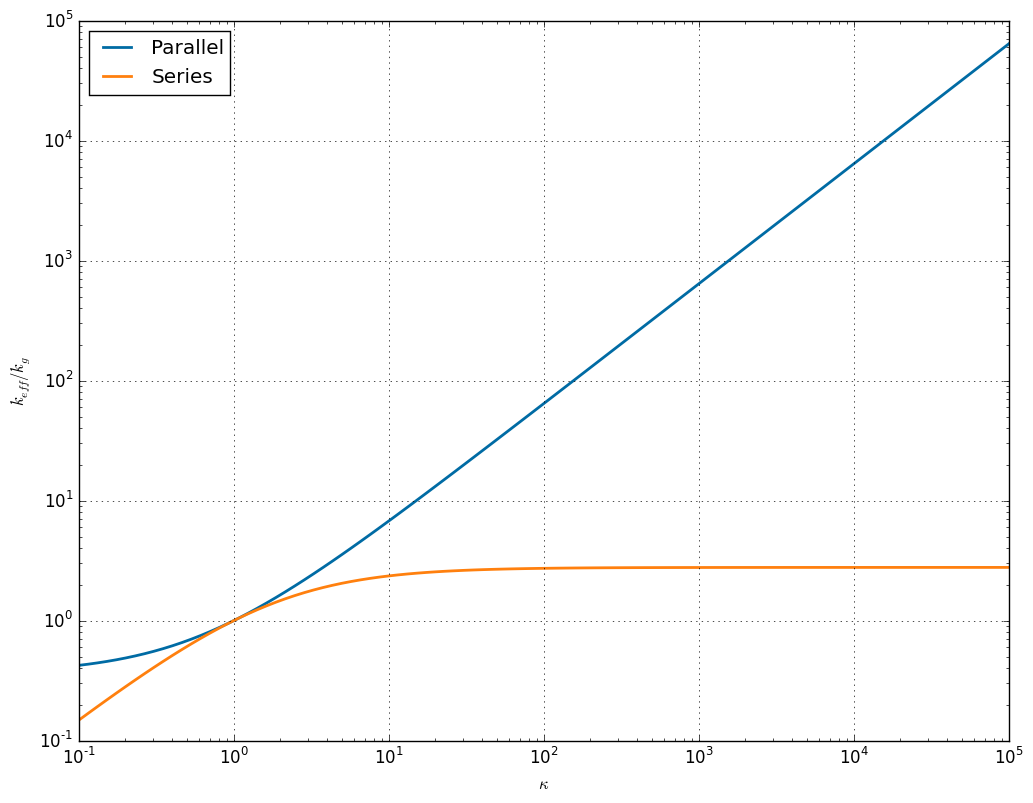
\includegraphics[width=\singleimagewidth]{figures/keff-kappa-series-parallel}
%     \caption{Upper and lower bounds of effective thermal conductivity in two-phase porous media are given by parallel and series approximations of the material, respectively.}
%     \label{fig:kappa-series-parallel}
% \end{figure}

One of the most widely-used correlations was put forth by Zehner and Schlunder in 1970 \cite{Zehner1970,Zehner1972}. They considered a cylindrically-shaped unit cell and made the analogy between heat and mass transfer to derive an empirical fit to data in the bulk of two-phase porous media. The Zehner-Schlunder (ZS) correlation is
\begin{equation}
    \frac{k_e}{k_f} = \left(1-\sqrt{1-\epsilon}\right)+\frac{2\sqrt{1-\epsilon}}{1-B/\kappa}\left[\frac{(1-1/\kappa)B}{(1-B/\kappa)^2}\ln\left( \frac{\kappa}{B} \right) - \frac{B+1}{2} - \frac{B-1}{1-B/\kappa}\right]
\end{equation}
where $B$ is a deformation parameter related to porosity as
\begin{equation}\label{eq:zs-B}
    B = 1.25\left(\frac{1-\epsilon}{\epsilon}\right)^{1.11}
\end{equation}

% The Zehner-Schlunder correlation is added to a figure with the parallel and series bounds

% \begin{figure}[!h]
%     \centering
%     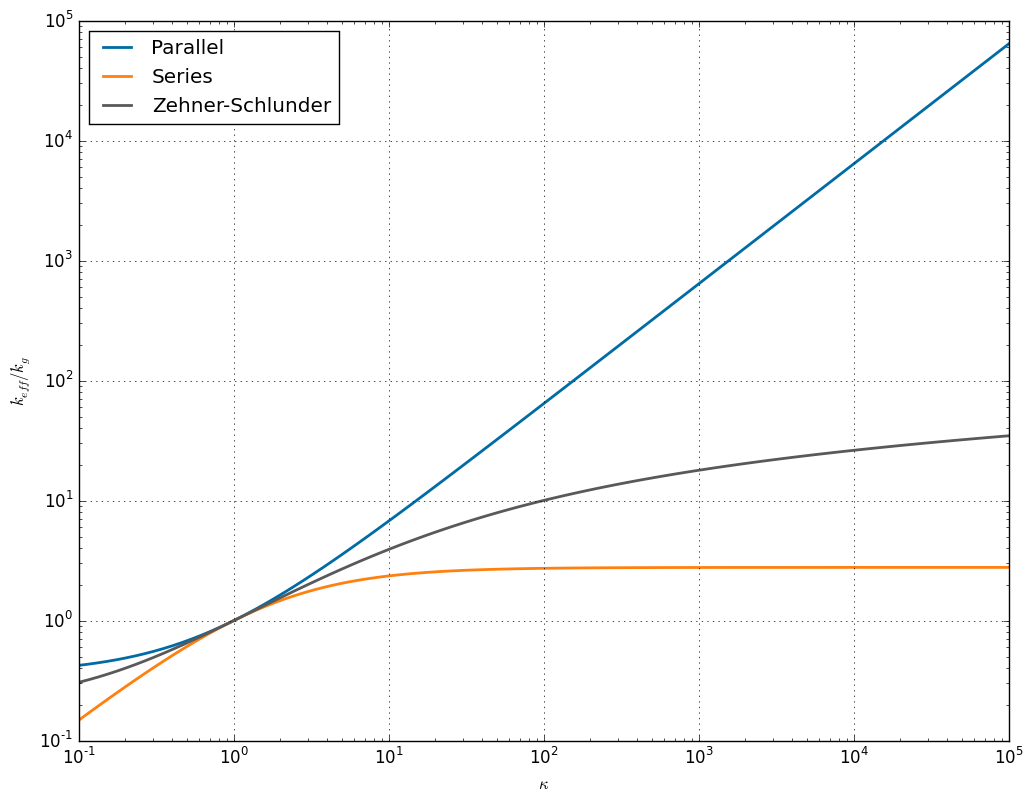
\includegraphics[width=\singleimagewidth]{figures/keff-kappa-series-parallel-zs}
%     \caption{Zehner-Schlunder correlation fitting between the upper and lower bounds of effective thermal conductivity in two-phase porous media are given by parallel and series approximations of the material, respectively.}
%     \label{fig:kappa-series-parallel-zs}
% \end{figure}

Following the success of the Zehner-Schlunder correlation, other researchers considered the specialized cases of high thermal conductivity ratio $\kappa \ge 10^3$ when loads on the grains in the bed (due to either an external pressure or the grains own weight) resulted in large contact areas. In these cases, Zehner-Schlunder correlations under-predicted the actual effective conductivity \cite{Aichlmayr2005a}. An extensive review of correlations for effective thermal conductivity with consideration of contact between grains is provided by van Antwerpen\etal \cite{VanAntwerpen2010}. Hsu\etal~considered three lumped parameters models of varying two-dimensional unit cells for which they derived an effective conductivity. The first was for contact square-cylinders. The effective conductivity for this model is
\begin{equation}
    \frac{k_e}{k_f} = \gamma_a\gamma_c\kappa + \frac{\gamma_a(1-\gamma_c)}{1+(1/\kappa-1)\gamma_a} + \frac{(1-\gamma_a)}{1+(1/\kappa-1)\gamma_a\gamma_c}
\end{equation}
where Hsu\etal~used the same fitting parameter of Nozad\etal, $\gamma_c$ \cite{nozad}; they found best agreement with experimental data when $\gamma_c = 0.01$. The other geometric parameter is related to $\gamma_c$ and $\epsilon$ as
\begin{equation}
    0=\gamma_a^2 + 2\gamma_a\gamma_c(1-\gamma_a) + \epsilon - 1
\end{equation}
Hsu\etal's second correlation had the square-cylinder unit cell replaced with circular-cylinders. The correlation is given with dependence on conductivity ratios. For $(1/\kappa-1)\gamma_a < 1$,
\begin{equation}
\begin{split}
    \frac{k_e}{k_f} ={} &\gamma_c\gamma_a\kappa + \frac{1-\gamma_a\sqrt{1-\gamma_c^2}}{\gamma_a\gamma_c(1/\kappa-1)+1} + \frac{\kappa(\pi/2 - 2\theta_c)}{1-\kappa} - \frac{2\kappa}{(1-\kappa)\sqrt{1-(1/\kappa-1)^2\gamma_a^2}}\\
    &\times\left[\tan^{-1}\left(\frac{\tan(\pi/4 - \theta_c/2)+(1/\kappa-1)\gamma_a}{\sqrt{1-(1/\kappa-1)^2\gamma_a^2}} \right) - \tan^{-1}\left(\frac{\tan(\theta_c/2)+(1/\kappa-1)\gamma_a}{\sqrt{1-(1/\kappa-1)^2\gamma_a^2}}\right) \right]
\end{split}
\end{equation}
For $(1/\kappa-1)\gamma_a>1$,
\begin{equation}
\begin{split}
    \frac{k_e}{k_f} ={} &\gamma_c\gamma_a\kappa + \frac{1-\gamma_a\sqrt{1-\gamma_c^2}}{\gamma_a\gamma_c(1/\kappa-1)+1} + \frac{\kappa(\pi/2 - 2\theta_c)}{1-\kappa} - \frac{\kappa}{(1-\kappa)\sqrt{(1/\kappa-1)^2\gamma_a^2-1}}\\
    & \times\left[\ln\left(\frac{\tan(\pi/4 - \theta_c/2)+(1/\kappa-1)\gamma_a - \sqrt{(1/\kappa-1)^2\gamma_a^2-1}}{\tan(\pi/4-\theta_c/2) +(1/\kappa-1)\gamma_a+\sqrt{(1/\kappa-1)^2\gamma_a^2-1}} \right) \right.\\
    & -\left.\ln\left(\frac{\tan(\theta_c/2)+(1/\kappa-1)\gamma_a - \sqrt{(1/\kappa-1)^2\gamma_a^2-1}}{\tan(\theta_c/2) +(1/\kappa-1)\gamma_a+\sqrt{(1/\kappa-1)^2\gamma_a^2-1}} \right) \right]
\end{split}
\end{equation}
and for $(1/\kappa-1)\gamma_a=1$
\begin{equation}
    \frac{k_e}{k_f} = \frac{\gamma_c\gamma_a^2}{\gamma_a+1}+\frac{1-\gamma_a\sqrt{1-\gamma_c^2}}{\gamma_c+1}+\gamma_a(\pi/2-2\theta_c)-\tan(\pi/4-\theta_c/2)+\tan(\theta_c/2)
\end{equation}
where $\gamma_c = 0.01$ was again found to fit best to experimental data. And the other geometric parameter relationship became
\begin{equation}
    0 = 1-\gamma_a\gamma_c-\frac{\gamma_a^2}{2}\left(\frac{\pi}{2}-2\theta_c\right)
\end{equation}
where the contact angle is $\theta_c = \sin^{-1}(\gamma_c)$.
The last correlation of Hsu\etal~came from three-dimensional unit cell extension of the square-cylinder to cubes,
\begin{equation}
    \frac{k_e}{k_f} = 1-\gamma_a^2 - 2\gamma_a\gamma_c + 2\gamma_a^2\gamma_c + \gamma_a^2\gamma_c^2\kappa + \frac{\gamma_a^2-\gamma_a^2\gamma_c^2}{1-\gamma_a + \gamma_a/\kappa} + \frac{2(\gamma_a\gamma_c - \gamma_a^2\gamma_c)}{1-\gamma_a\gamma_c+\gamma_a\gamma_c/\kappa}
\end{equation}
where $\gamma_c = 0.13$ fit best for cubes and the relationship between $\gamma_c$, $\epsilon$\ and $\gamma_a$ became
\begin{equation}
    0 = (1-3\gamma_c^2)\gamma_a^3 + 3\gamma_c^2\gamma_a^2 + \epsilon - 1
\end{equation}

Hsu\etal~also proposed a correction to the ZS model for conductivity ratios of $\kappa \ge 10^3$. The assumption built into Zehner-Schlunder's model was of a point contact between grains in the bed. Incorporating the effects of finite-sized contact area, Hsu\etal~corrected the ZS model as
\begin{equation}
\begin{split}
    \frac{\kappa_e}{\kappa_f}={} &(1-\sqrt{1-\epsilon}) + \kappa\sqrt{1-\epsilon}\left(1-\frac{1}{(1+\alpha_0B)^2}\right) \\
    & + \frac{2\sqrt{1-\epsilon}}{1-B/\kappa + (1-1/\kappa)\alpha_0B}\left[\frac{(1-1/\kappa)(1+\alpha_0)B}{(1-B/\kappa + (1-1/\kappa)\alpha_0B)^2}\ln\left[\frac{1+\alpha_0B}{(1+\alpha_0)B/\kappa}\right] \right.\\
    & - \left.\frac{B+1+2\alpha_0B}{2(1+\alpha_0B)^2} - \frac{B-1}{(1-B/\kappa+(1-1/\kappa)\alpha_0B)(1+\alpha_0B)} \right]
\end{split}
\end{equation}
where $B$ is no longer found from as a simple deformation parameter but is instead related to $\epsilon$ and $\alpha_0$. Hsu\etal~found best agreement with experimental data when $\alpha_0 = 0.002$ and $\epsilon=0.42$. $B$ can then be found from the solution of
\begin{equation}
\begin{split}
    0 ={} & 1-\frac{B^2}{(1-B)^6(1+\alpha_0B)^2}\bigg[(B^2-4B+3)+2(1+\alpha_0)(1+\alpha_0B)\ln\left(\frac{(1+\alpha_0)B}{1+\alpha_0B}\right)\\
    &+\alpha_0(B-1)(B^2-2B-1)\bigg]^2 - \epsilon
\end{split}
\end{equation}

Bauer and Schlunder \cite{bauer1978effective} also improved on the earlier model of Zehner and Schlunder to include the additional effects of thermal radiation, gas heat transfer in the Knudsen regime, and finite-sized contact areas. The combined model, often called the Zehner-Bauer-Schlunder (ZBS) model is calculated as
\begin{equation}
    \frac{k_e}{k_f} = \left(1-\sqrt{1-\epsilon}\right)\epsilon\left[\left(\epsilon-1+1/\kappa_G\right)^{-1} + \kappa_r\right]+\sqrt{1-\epsilon}\left(\phi\kappa + (1-\phi)k_c\right)
\end{equation}
where
\begin{equation}
\begin{split}
    k_c ={} &\frac{2}{N}\left[\frac{B(\kappa+\kappa_r -1)}{N^2\kappa_G\kappa}\ln\left(\frac{\kappa+\kappa_r}{B(\kappa_G+(1-\kappa_G)(\kappa+\kappa_r))}\right) \right.\\
    &+\left.\frac{B+1}{2B}\left(\frac{\kappa_r}{\kappa_G} - B\left(1+\frac{1-\kappa_G}{\kappa_G}\kappa_r\right) \right) - \frac{B-1}{N\kappa_G}\right]
\end{split}
\end{equation}
and
\begin{equation}
    N = \frac{1}{\kappa_G}\left(1+\frac{\kappa_r-B\kappa_G}{\kappa} \right) - B(1-1/\kappa_G)(1+\kappa_r/\kappa)
\end{equation}
and $B$ is given in \Cref{eq:zs-B}. Radiation is incorporated in $\kappa_r$ parameter, given as
\begin{equation}
    \kappa_r = \frac{4\sigma}{2/\epsilon_r - 1}\bar{T}^3\frac{d_p}{k_f}
\end{equation}
where $\sigma$ is the Stefan-Boltzmann number ($\sigma = $~\SI{5.67e-8}{\watt\per\meter\squared\per\kelvin\tothe{4}}), $\epsilon_r$ is the emissivity of the material in the packing, $d_p$ is the packing diameter (assumed spherical), and $\bar{T}$ is the average, absolute temperature of the system (in \si{\kelvin}). 

Effects due to interstitial gas in the Knudsen regime are defined by the term, $\kappa_G$ given as
\begin{equation}
    \kappa_G = \left[1 + \left(\frac{l}{d_p}\right)\right]^{-1}
\end{equation}
where $l$ is a modified mean free path of gas molecules,
\begin{equation}
    l = 2\frac{2-\alpha_T}{\alpha_T}\left(\frac{2\pi\tilde{R}\bar{T}}{M_g}\right)^{1/2}\cdot\frac{k_f}{P(2c_p - \tilde{R}/M_g)}
\end{equation}
where $P$ is the gas pressure (in \si{\pascal}), $\tilde{R}$ is the universal gas constant (in \si{\joule\per\mol\per\kelvin}), and $M_g$ is the molecular mass of the gas (in \si{\kilo\gram\per\mol}). The accommodation factor, $\alpha_T$ is given by Bahrami\etal~(originally given by Song \& Yovanovich) as \cite{Bahrami20063691,song1988relative}
\begin{equation}
    \alpha_T = \exp\left[-0.57T_r\right]\left(\frac{M^*}{6.8+M^*}\right) + \frac{2.4\mu}{(1+\mu)^2}\left[1-\exp\left(-0.57T_r\right)\right]
\end{equation}
where $T_r = \frac{T_s-\SI{273}{\kelvin}}{\SI{273}{\kelvin}}$, $M^* = M_g$ for monatomic gases or $M^* = 1.4M_g$ for diatomic gases, and $\mu = \frac{M_g}{M_s}$ is the ratio of gas and solid molecular masses. The $\alpha_T$ term, as described by Bahrami\etal~ represents the fraction of kinetic energy that a gas molecule leaves behind as thermal energy on a solid after collision.

In \Cref{fig:kappa-series-parallel-zs-hsus}, we see comparisons of effective conductivity predictions by the three models of Hsu\etal~, Hsu\etal~ modification of ZS model, ZSB correction model, and their differences with the simple ZS correlation.

\begin{figure}[!h]
    \centering
    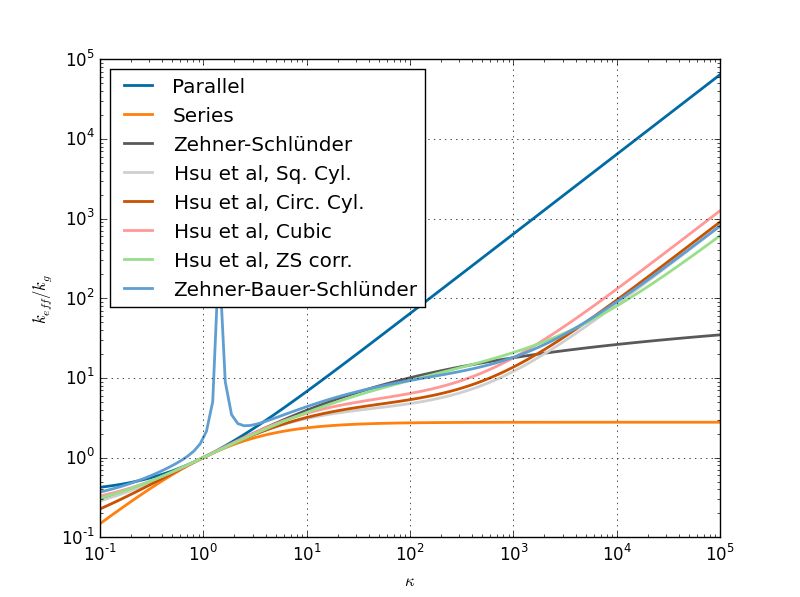
\includegraphics[width=\singleimagewidth]{figures/keff-kappa-series-parallel-zs-hsus}
    \caption{Models incorporating contact area demonstrate signficant deviation from the Zehner-Schlunder correlation above $\kappa > 10^3$. All correlations are still bound by parallel and series approximations of the material.}
    \label{fig:kappa-series-parallel-zs-hsus}
\end{figure}

Van Antwerpen compiled data from numerous publications to compare the accuracy of effective conductivity correlations \cite{VanAntwerpen2010}. For our discussion, I have also plotted the experimental data with all the correlations discussed above, given in \Cref{fig:kappa-experimental}.

Near $\kappa = 1$, all correlations collapse to predict a $\frac{k_e}{k_f} = 1$, and experiments naturally match predictions. From the range of $\kappa > 1$ to $\kappa <1000$, experimental data is well-bound by the predictions of the simple ZS model and the complex two-dimensional models of Hsu\etal. Above $\kappa > 1000$, the ZS model, not taking into account heat transfer through finite-sized contacts, is no longer reliable as a model for $\keff$. In high ranges of $\kappa$, the models incorporating contact-conduction in the granular material remain well-matched to experimental data. The results here show the worth of these general models for predictions of effective conductivity in some granular material.

\begin{figure}[!h]
    \centering
    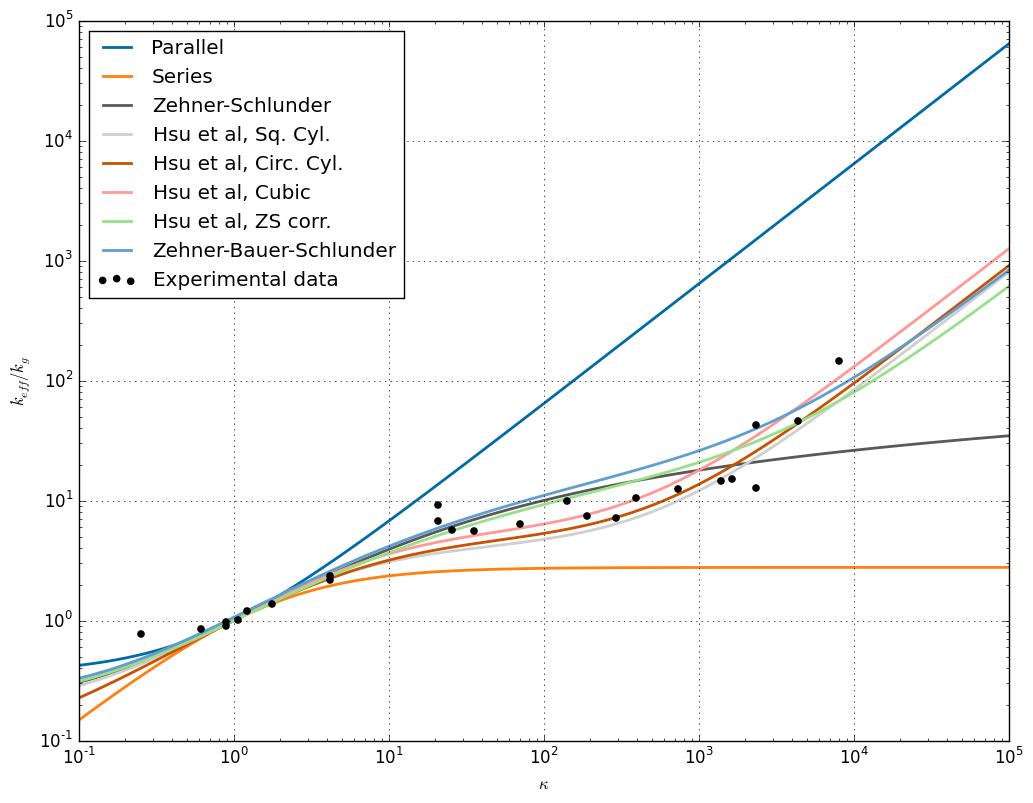
\includegraphics[width=\singleimagewidth]{figures/keff-kappa-experimental}
    \caption{Comparison of $\keff$ correlations with compiled experimental data over a broad range of conductivity ratios, $\kappa$. Data compiled by \cite{VanAntwerpen2010} from many sources.}
    \label{fig:kappa-experimental}
\end{figure}

As part of the Ceramic Optimal Material Experiments for Thermomechanics (COMET) project at UCLA, we measured the effective conductivity of $d_p = $~\SI{1}{\milli\meter} graphite (IG11) pebbles for \SIrange{135}{544}{\celsius}. The results will be discussed in more detail later, though the results will be presented here for comparison with the correlations; \Cref{fig:kappa-experimental-comet} shows the COMET data. The measured conductivity from COMET is well above the lower bounds of series approximation for effective conductivity, though is just below the lowest values predicted from Hsu\etal's square-cylinder two-dimensional model. As will be discussed in \Cref{sec:granular-contact-roughness}, we attribute the smaller values of effective conductivity on the surface roughness of the graphite pebbles in conjunction with their small size and small mass. In short, however, the measurements of COMET are also demonstrative of the inaccuracies in general predictions of granular material thermal properties.

\begin{figure}[!h]
    \centering
    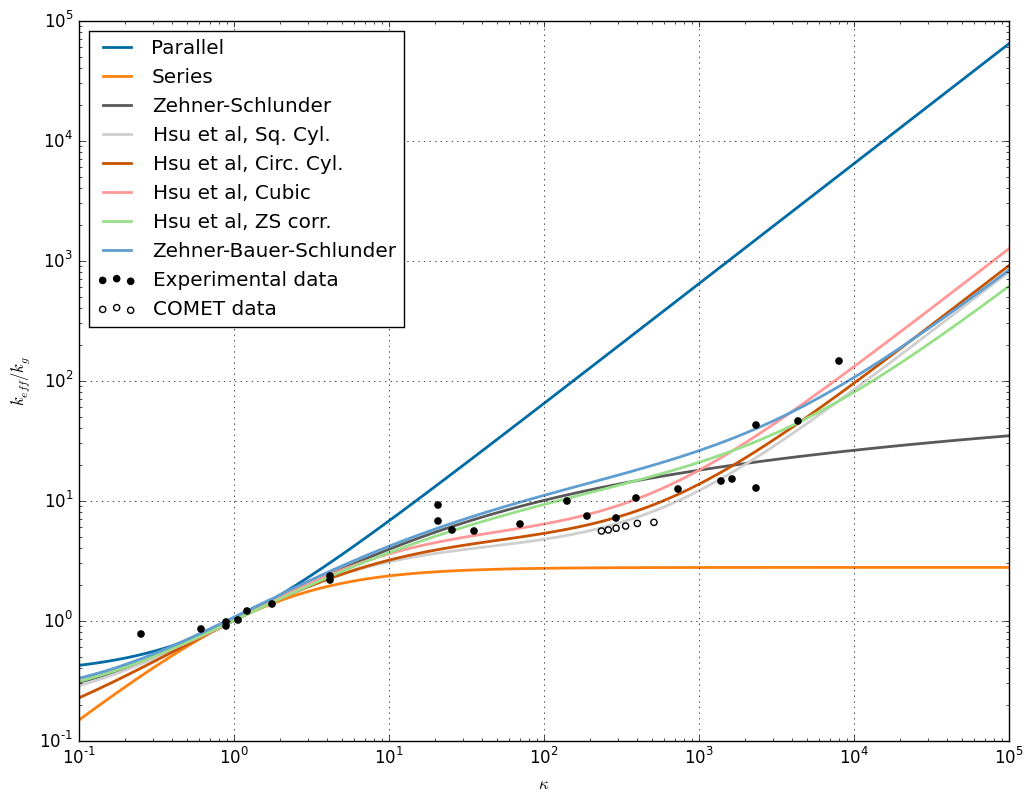
\includegraphics[width=\singleimagewidth]{figures/keff-kappa-experimental-comet}
    \caption{Comparison of COMET data on IG11 graphite, $\keff$ correlations, and experimental data. Data compiled by \cite{VanAntwerpen2010} from many sources and measured data at UCLA.}
    \label{fig:kappa-experimental-comet}
\end{figure}












%~~~~~~~~~~~~~~~~~~~~~~~~~~~~~~~~~~~~~~~~~~~~~~~~~~~~~~~~~~~~~~~~~~~~~~~~~~~~~~~~~~~~~~~~~~~~~~~~~~~~~~~~~~~
% new subsection
%~~~~~~~~~~~~~~~~~~~~~~~~~~~~~~~~~~~~~~~~~~~~~~~~~~~~~~~~~~~~~~~~~~~~~~~~~~~~~~~~~~~~~~~~~~~~~~~~~~~~~~~~~~~
\subsection{Convection in Granular Media}\label{sec:particle-convection}
Before discussing the correlations for Nusselt number of particles with forced convection in two-phase porous media, I will consider a simple case of an axisymmetric sphere completely immersed in a quiescent fluid. The steady-state energy equation of the fluid surrounding the sphere is 
\begin{equation}
    \frac{\partial}{\partial}(k_fr^2T) = 0
\end{equation}
for which the solution is 
\begin{equation}
    T = -\frac{C_1}{r} + C_2
\end{equation}
subjected to a boundary condition of
\begin{equation}
    k_f\frac{\partial T}{\partial r}\Bigg|_R = -h(T_R - T_f)
\end{equation}
where $T_R$ is the temperature of the fluid in contact of the sphere of radius $R$ and $T_f$ is the temperature of the fluid infinitely far away from the sphere -- which naturally leads to the second boundary condition of $T(r\rightarrow\infty) = T_f$. These two boundary conditions yield a temperature solution of 
\begin{equation}
    T = \frac{hR}{k_f}\frac{R}{r}(T_R -T_f) + T_f
\end{equation}
We can also say $T(r = R) = T_R$ to show,
\begin{equation}
    T_R = \frac{hR}{k_f}\frac{R}{R}(T_R -T_f) + T_f
\end{equation}
or simply
\begin{equation}
    \frac{hR}{k_f} = 1
\end{equation}
The Nusselt number for a sphere is defined as
\begin{equation}
    \Nu_p = \frac{hd_p}{k_f}
\end{equation}
which is simply
\begin{equation}
    \Nu_p = 2\frac{hR}{k_f} = 2
\end{equation}
showing that in the limit of $\Re_p \rightarrow 0$, the Nusselt number for a sphere in fluid will asymptotically approach $\Nu_p = 2$. This value is a natural limit for a Nusselt number correlation for particle-to-fluid heat transfer. 

\subsubsection{Nusselt number correlations for an individual sphere}
For a particle falling through a fluid or a fluid moving past a single particle, a number of correlations exist for the Nusselt number of that individual sphere. One common correlation is from Ranz \& Marshall\cite{Ranz1952}, developed from heat and mass transfer analogies with experiments on evaporating drops. Their correlation is
\begin{equation}\label{eq:ranz_marshall}
    \Nu_p = 2.0 + 0.6\Pr^{1/3}\Re_p^{1/2}
\end{equation}
Generally considered valid for $\Re_p< 200$. The Ranz \& Marshall correlation is used by Sasdisevi\etal~ in a CFD-DEM study of heat transfer in 2D fluidized spouts \cite{Swasdisevi2005}. Romkes\etal~ did direct CFD studies of particle-to-fluid heat transfer and validated against Ranz \& Marshall \cite{Romkes2003}; though they noted the correlation was valid over particle Reynolds numbers of $10 < \Re_p < 10^4$. Wu\etal~ also employed the correlation in a DEM study of granular material\cite{Wu2011}. Li \& Mason studied the correlation against their CFD-DEM studies \cite{Li2003a}, they found the RM correlation to be adequate for small $\Re_p < 200$ also. 



Gnielinski\cite{gnielinski1982berechnung} developed a semi-empirical method where the Nusselt number for an arbitrary shape is related to the solution for a flat plate with appropriate transformations of the length scale. The solution is a function of the asymptotic laminar, turbulent, and $\Re_p\rightarrow 0$ solutions,
\begin{equation}\label{eq:gnielinski}
    \Nu_p = 2 + \sqrt{\Nu^2_{lam} + \Nu^2_{tur}}
\end{equation}
where
\begin{equation}
    \Nu_{lam} = 0.664\Re_p^{1/2}\Pr^{1/3}
\end{equation}
and
\begin{equation}
    \Nu_{turb} = \frac{0.037 \Re_p^{0.8}\Pr}{1 + 2.443\Re_p^{-0.1}(\Pr^{2/3}-1)}
\end{equation}


The two single-particle correlations are shown over a range of Reynolds numbers in \Cref{fig:Nu-single}. The two correlations are in good agreement near low Reynolds number.

\begin{figure}[!h]
    \centering
    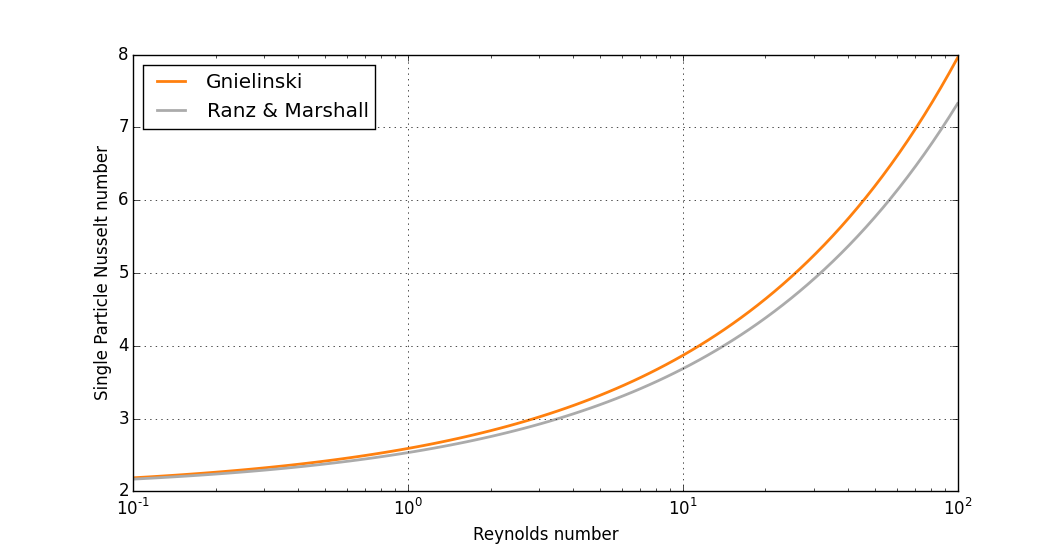
\includegraphics[width=\singleimagewidth]{figures/Nusselt-single}
    \caption{Comparison of correlations for Nusselt number of a single spherical particle in forced flow.}
    \label{fig:Nu-single}
\end{figure}





\subsubsection{Nusselt number correlations for a sphere as part of a packing}
However, this correlation was developed from measurements of a single particle in flow. The influence of neighboring grains will disrupt the flow field and result in a different Nusselt number. Thus, for the Nusselt number for a single grain in a packed bed, $\Nu_i$, is often related to the Nusselt number of a single particle (alone in an infinite fluid), $\Nu_p$, via the packing fraction. The subscripts $i$ and $p$ will be used consistently below to signify the Nusselt for a particle in a packing or a correlation for a single particle. 

The data of Ranz suggested the following for spherical particles in a fixed bed
\begin{equation}\label{eq:ranz-packing}
    \Nu_i = 2 + 1.8\Re_p^{0.6} \Pr^{1/3}
\end{equation}

Another commonly-cited correlation is that of Wakao\etal~\cite{Wakao1978,wakao1982heat}. Combining a large amount of data over a broad range of particle Reynolds numbers and Prandlt numbers found a fitting function of
\begin{equation}\label{eq:wakao}
    \Nu_i = 2 + 1.1\Re_p^{0.6} \Pr^{1/3}
\end{equation}
Flueckiger\etal \cite{Flueckiger2014,Flueckiger2011a,Flueckiger2011} as well as Yang \& Garimella\cite{Yang2010}, both implemented the Wakao\etal~ correlation in their studies of heat transfer in solar thermal storage tanks. 

Zhou\etal\cite{Zhou2009} used a modified form from Kunii and Levenspiel, to fit their experimental data. They gave
\begin{equation}\label{eq:kunii}
    \Nu_i = 2 + 1.2\Re_p^{1/2}\Pr^{1/3}
\end{equation}

In another study, Li \& Mason\cite{Li2000} also employed a modified form of Ranz \& Marshall to account for the packing in the assembly with a function of void fraction in front of the Reynolds and Prandtl terms,
\begin{equation}\label{eq:modified-ranz}
    \Nu_i = 2+ 0.6\epsilon^n\Re_p^{1/2}\Pr^{1/3}
\end{equation}
where they found $n= 3.5$ fitting for \SI{3}{\milli\meter} pellets in dilute flows\cite{Li2000}. Kloss\etal~\cite{Kloss2012} and Di Maoi\etal\cite{DiMaio2009} also use the modified Ranz \& Marshall correlation provided by Li \& Mason in their CFD-DEM studies. This correlation, however, conflicts with the correlations of Ranz, Wakao, and the Kunii \& Levenspiel. In the asymptotic limit of $\epsilon \rightarrow 1$, the correlation correctly approaches the single particle correlation of Ranz \& Marshall, \Cref{eq:ranz_marshall}. For a dense packing, $\epsilon = 0.36$, the correlation gives
\begin{equation}
    \Nu_i = 2+ 0.0168\Re_p^{1/2}\Pr^{1/3}
\end{equation}
which is significantly less than any of the correlations of \Cref{eq:ranz-packing,eq:wakao,eq:kunii}


Achenbach defined an empirical arrangement factor, $f(\epsilon) = 1+1.5(1-\epsilon)$ to related the single particle $\Nu$ of Gnielinski, \Cref{eq:gnielinski}, to a sphere in a packing,
\begin{equation}\label{eq:modified-gnielinski}
    \Nu_i = \left(1 + 1.5(1-\epsilon)\right)\Nu_p
\end{equation}
The modified form of Achenbach was used in a CFD-DEM study by Rickelt\etal \cite{Rickelt2013}, which covers $\Re_p$ up to \num{10e5} and $\Pr$ from \numrange{0.7}{7e4}. The Gnielinski correlation\cite{gnielinski1982berechnung} is also used in the ANSYS calculations of helium-cooled pebble bed breeders, reported by Hernandez\etal\cite{Hernandez2013}, Cismondi\etal\cite{Cismondi2009}, Poitevin\etal\cite{Poitevin2010}, \textit{etc.} However, Visser notes \cite{Visser2007} that the correlation of Gnielinksi is valid for $\Re_p$ in \numrange{500}{1000}, for $\epsilon$ in the range \numrange{0.26}{1.0}. Thus he uses the correlation of Gunn for his situation of lower Reynolds number\cite{Gunn1978}
\begin{equation}\label{eq:gunn}
    \Nu_i = (7-10\epsilon+5\epsilon^2)(1+0.7\Re_p^{0.2}\Pr^{1/3})+(1.33-2.4\epsilon+1.2\epsilon^2)\Re_p^{0.7}\Pr^{1/3}
\end{equation}
which Gunn developed to be valid for: heat transfer to particles at low and high Reynolds number, at low and high porosities; single particle at low Reynolds number, particles and particles in ensembles with high Reynolds number and moderate Prandtl. Amritkar\etal~also employ the Gunn correlation in their simulations of spout-fluidized flow \cite{Amritkar2014}.

The correlations are given as functions of $\Re$ at a specified value of $\epsilon = 0.36$ and $\Pr = 0.7$ in \Cref{fig:Nu-packed}. We see the correlation from Li \& Mason (a modified form of Ranz \& Marshall), from \Cref{eq:modified-ranz}, predicts very small Nusselt numbers over this entire range of Reynolds number. Additionally, the modified Gnielinski of \Cref{eq:modified-gnielinski} and the correlation of Gunn in \Cref{eq:gunn} predict much higher Nusselt numbers at low Reynolds number than any other correlation, and are well above the single particle limit of $\Nu = 2$ when $\Re \rightarrow 0$. In the studies of Achenbach and Rickelt, which employed the modified Gnielinski studies, the authors were interested in larger Reynolds number regimes. Above $\Re > 10$, Gnielinski correlation is similar to Wakao and Ranz correlations, thus the over-prediction at very small $\Re$ may not have been observed. Gunn rejects the notion that the Nusselt number should approach 2 in the no-flow limit \cite{Gunn1978}. The discrepancy appears to arise because of definitions of either particle or bed heat transfer coefficients. It seems Gunn's definition was meant for representative cross sections of packed beds with voidage defined by the void fraction rather than for an individual particle communicating with forced flow in a packed bed. 

\begin{figure}[!h]
    \centering
    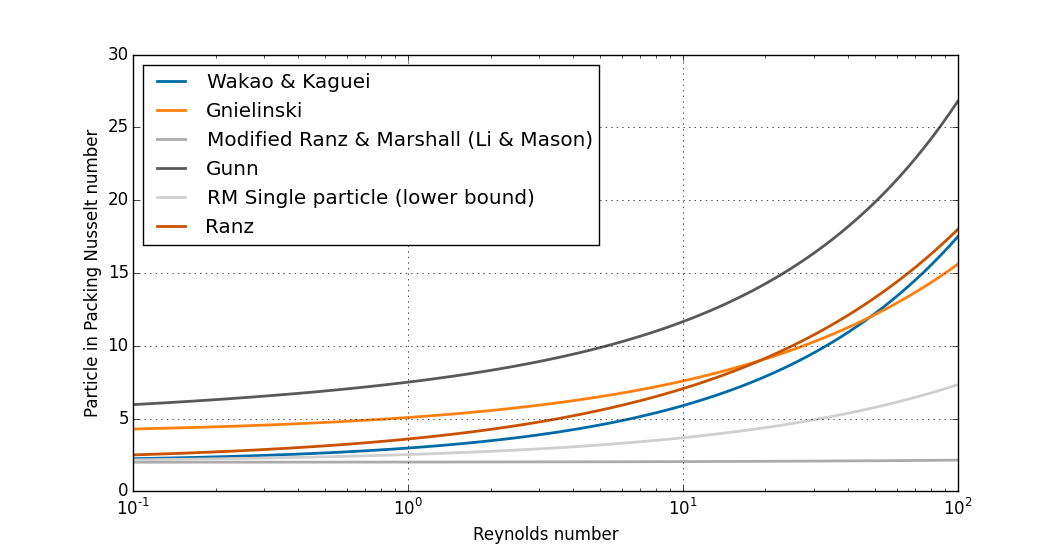
\includegraphics[width=\singleimagewidth]{figures/Nusselt-packing}
    \caption{Comparison of correlations for Nusselt number of a single spherical particle in forced flow.}
    \label{fig:Nu-packed}
\end{figure}

After discussing many popular correlations for Nusselt number in packed beds, considering the very small Reynolds number ($\Re \sim 1$) and packing fraction expected with the purge gas of helium in tritium breeders, the correlation of Wakao\etal, as given in \Cref{eq:wakao}, is sufficient. However, we note the debate that still exists in literature for determining Nusselt number for a specific particle in a packed bed. If experimental validation shows the Wakao correlation to be inaccurate, we will revisit the implementation in our modeling.

% Whitaker in 1972 \cite{Whitaker1972}
% Definition of Reynolds number
% \begin{equation}
%   \Re = \frac{D_p G}{\mu_b(1-\epsilon)}
% \end{equation}
% Definition of Nusselt number
% \begin{equation}
%   \Nu = \frac{hD_p}{k_f}\frac{\epsilon}{1-\epsilon}
% \end{equation}
% Definition of h
% \begin{equation}
%   h_{\ln} = \frac{\dot{Q}}{a_v}V\Delta T_{\ln}
% \end{equation}
% where $a_v = (A_p/V_p)(1-\epsilon)$ is the surface area per unit volume. And $\delta T_{\ln}$ is the log-mean temperature difference.
% Reference temp, $T^*$
% \begin{equation}
%   T^* = \frac{1}{2}(T_{f1} + T_{f2})
% \end{equation}
% Range of Reynolds number
% $22-8 \times 10^3$
% Range of Prandtl number
% 0.7
% Range of ($\mu_b/\mu_0$)
% 1
% Correlation,
% \begin{equation}
%   \Nu = \left( 0.5 \Re^{1/2} + 0.2\Re^{2/3} \right)\Pr^{1/3}
% \end{equation}





% Gao\etal used thermal lattice-Boltzmann simulations to develop Nusselt number correlations in porous media with natural convection\cite{Gao2014}














% Romkes\etal~ show generalized forms of Nusselt number of the form
% \begin{equation}
%     \Nu = c_1 + c_2\Re^{n}\Pr^{1/3}
% \end{equation}
% where the constants are defined based on the style of packing. They consider
% \begin{enumerate}
% \item particle-to-fluid heat transfer of a single free sphere in a static infinite medium
% \item particle-to-fluid heat transfer of a single free sphere in a flowing fluid
% \item wall-to-fluid heat transfer of an empty channel with laminar flow
% \item wall-to-fluid heat transfer of an empty channel with turbulent flow
% \item particle-to-fluid heat transfer of a tube filled with catalyst particles
% \end{enumerate}

% For (1), $\Nu = 2$ in steady-state. For (3), in a fully-developed region, $\Nu = 3.66$ for constant temperature boundary conditions and $\Nu = 4.36$ for constant heat flux boundary conditions. 

% Romkes\etal~give Ranz \& Marshall, Whitaker, and Achenbach correlations, respectively, as correlations for (2) when there is an infinite medium surrounding a single sphere
% \begin{equation}
%     \Nu = 2 + 0.66\Re^{0.5}\Pr^{0.33}
% \end{equation}
% for $\Re$ in the range \numrange{10}{1e4}, and $\Pr > 0.7$. (assuming $\Pe \gg 1$).
% \begin{equation}
%     \Nu = 2 + (0.4\Re^{0.5}+0.06\Re^{0.67})\Pr^{0.4}
% \end{equation}
% for $\Re$ in the range \numrange{3.5}{7.6e4}, and $\Pr$ in the range \numrange{0.7}{380}
% \begin{equation}
%     \Nu = 2.0 + \left(\frac{1}{4}\Re + \num{3e-4}\Re^{1.6}\right)
% \end{equation}
% for $\Re$ in the range \numrange{1e2}{2e5}

% Romkes\etal~give a `conventional engineering relation' for heat transfer in a randomly packed bed as
% \begin{equation}
%     \Nu = (1.8\pm 0.3)\Re^{1/2}\Pr^{1/3}
% \end{equation}
% for $\epsilon = 0.4$, $\Re$ in the range \numrange{30}{3e3}, and $\Pr \ge 1$. And he sites that $c_1$ in the above equation is dropped as in ERG Eckert from 1956 transactions of ASME 56, and Gnielinksi in a 1978 publication.





%~~~~~~~~~~~~~~~~~~~~~~~~~~~~~~~~~~~~~~~~~~~~~~~~~~~~~~~~~~~~~~~~~~~~~~~~~~~~~~~~~~~~~~~~~~~~~~~~~~~~~~~~~~~
% new subsection
%~~~~~~~~~~~~~~~~~~~~~~~~~~~~~~~~~~~~~~~~~~~~~~~~~~~~~~~~~~~~~~~~~~~~~~~~~~~~~~~~~~~~~~~~~~~~~~~~~~~~~~~~~~~
\subsection{Radiation in Granular Media}

The temperatures expected in the solid breeder are high enough radiation between grains may be important. The radiation exchange between contacting neighbors in a packed bed becomes extremely complex due to the local and semi-local nature of radiation. A standard approach to treat radiation exchange between surfaces is to consider the view factor between them. In a dense, randomly packed bed of spheres the computation of view factors between pebbles can be done via a method such as that proposed Feng and Han \cite{Feng2012}. 

The ZSB model incorporates radiation heat transfer into the general expression and calculation of $k_c$ and $N$. Others have attempted to incorporate radiation into an effective thermal conductivity and typically it is done with a superposition of gas/solid conduction models (such as all those described above) with a separate radiation model. One common technique is to analyze a representative unit cell with a thermal radiative conductivity of a general form,
\begin{equation}
     k_e^r = 4 F_E^*\sigma d_p \bar{T}^3
\end{equation} 
where $F_E^*$ is a radiation exchange factor. Van Antwerpen\etal~describe many researchers' techniques for defining the radiation exchange factors and the simplifications that must appear to allow a closed solution to complicated equations. I will focus on one commonly-used correlation from Breitbach \& Barthels \cite{breitbach1980radiant}.

Breitbach \& Barthels began with the unit cell defined by Zehner \& Schlunder, though noted that the closed cell precluded radiation from voids outside the cell volume. Therefore they modified the correlation via closing the bases of the unit cells with black surfaces instead of with surfaces of the same emissivity as the grains in the bed. The result is given as the BB correlation,\cite{breitbach1980radiant}
\begin{equation}
    F_E^* = \left[\left(1-\sqrt{1-\epsilon}\right)\epsilon + \frac{\sqrt{1-\epsilon}}{2/\epsilon_r - 1}\cdot\frac{B+1}{B}\cdot\frac{1}{1+\frac{1}{(2/\epsilon_r - 1)\Lambda_f}} \right]
\end{equation}
where $B$ is again given by \Cref{eq:zs-B}, and $\Lambda_f = \frac{k_s}{4d_p\sigma\bar{T}^3}$ is a dimensionless solid conductivity for the granular packing.


An IAEA technical report provides effective conductivity measurements of $d_p =$~\SI{60}{\centi\meter} graphite pebble beds\cite{Report2000}. The data is used to compare against the combined correlations of ZS and BB. The $\keff$ measurements in Helium are given in \Cref{fig:keff-sana-he}, measurements in Nitrogen are given in \Cref{fig:keff-sana-n}. We see that the effective thermal conductivity correlations are significantly under-predicting, over the entire range of temperatures, when compared to experimental values. For the graphite pebble beds measured in the SANA report, we consider the Grashof number for the packing. The Grashof number is indicative of natural convection effects in the voids. The Grashof number is written as
\begin{equation}
    \Gr = \frac{g\beta(T_s-T_0)l^3}{\nu_f^2}
\end{equation}
where we estimate it in voids of size $l = \frac{d_p}{2}$, a temperature drop of $T_s-T_0 = $~\SI{10}{\kelvin} is an lower estimate. The kinematic viscosity, $\nu_f$ of the gases is known, and thermal expansion of an ideal gas is $\beta = \frac{1}{T}$. Let us assume a situation where temperatures and materials are all identical and the only variation is in length. Grashof numbers for these cases would be
\begin{equation}
    \frac{\Gr_1}{\Gr_2} = \left(\frac{l_1}{l_2}\right)^3
\end{equation}

Zehner \& Schlunder derived their correlation from mass-diffusion experiments of Curie \cite{Currie2002}. The data of Curie was done primarily on grains of around \SI{1}{\milli\meter}. Thus comparing $\frac{l_1}{l_2}$ between the size of particles for which the ZS correlation was derived and particles for which it was applied for SANA data yields
\begin{equation}
    \frac{\Gr_1}{\Gr_2} \sim 10^{-6}
\end{equation}
With a Grashof number significantly higher for the SANA experiments, it is indicative that the amount of natural convection present in the SANA experiment will have a much greater impact on heat transfer than the ZS correlation, derived on data for stagnant inter-stitial gas, is able to predict. This demonstrates limited applicability of effective conductivity correlations for packed bed conditions different from those for which the correlations were derived.

\begin{figure}[!h]
    \centering
    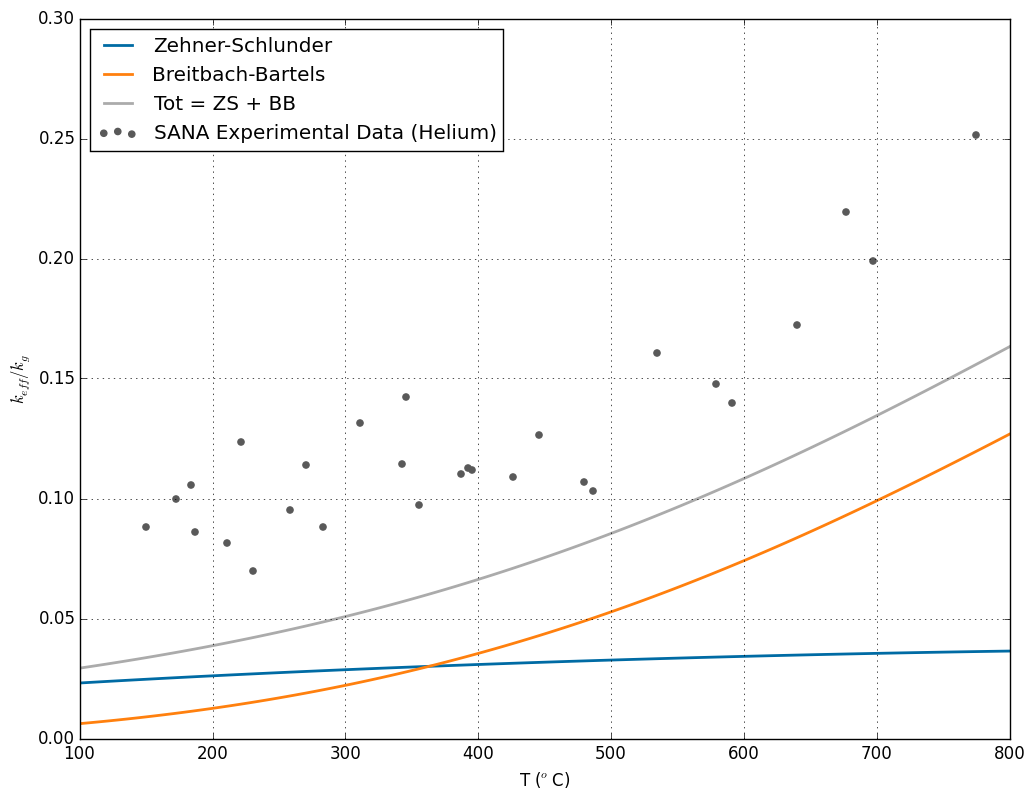
\includegraphics[width=\singleimagewidth]{figures/keff-sana-he}
    \caption{Comparison of SANA data in Helium gas with Zehner-Schlunder and Breitbach-Bartels correlations. Data from IAEA Tecdoc-1163\cite{Report2000}.}
    \label{fig:keff-sana-he}
\end{figure}
\begin{figure}[!h]
    \centering
    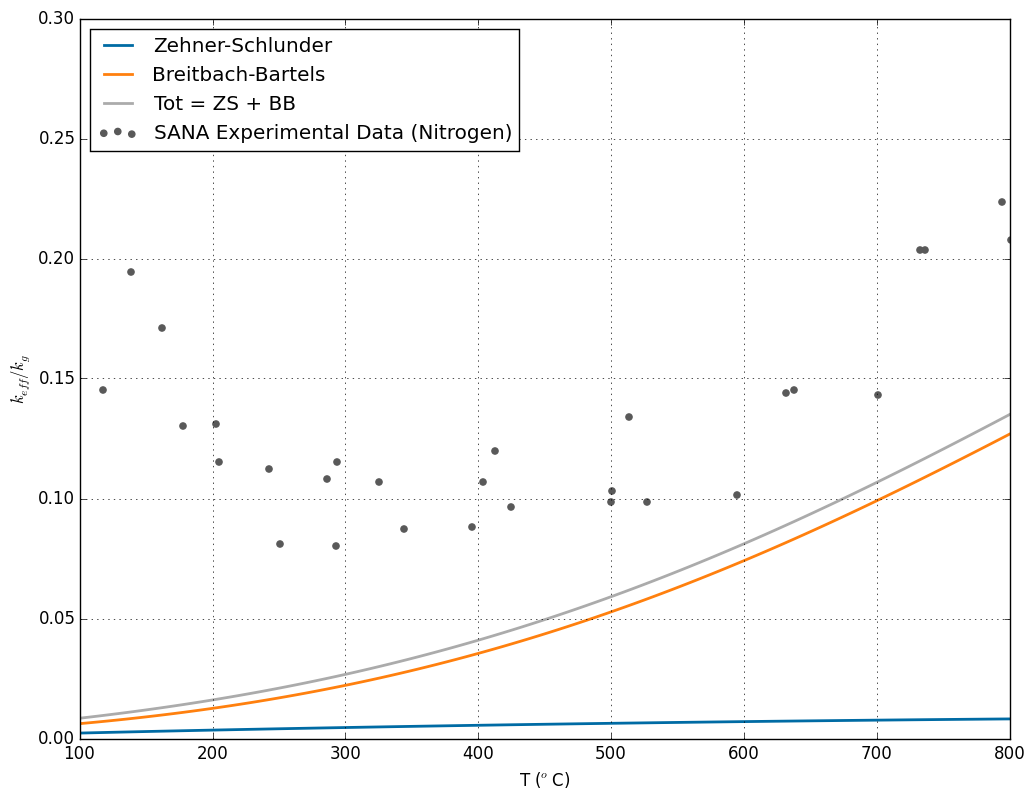
\includegraphics[width=\singleimagewidth]{figures/keff-sana-n}
    \caption{Comparison of SANA data in Nitrogen gas with Zehner-Schlunder and Breitbach-Bartels correlations. Data from IAEA Tecdoc-1163\cite{Report2000}.}
    \label{fig:keff-sana-n}
\end{figure}

\FloatBarrier



%%%%%%%%%%%%%%%%%%%%%%%%%%%%%%%%%%%%%%%%%%%%%%%%%%%%%%%%%%%%%%%%%%%%%%%%%%%%%%%%%%%%%%%%%%%%%%%%%%%%%%%%%%%%
%%%%%%%%%%%%%%%%%%%%%%%%%%%%%%%%%%%%%%%%%%%%%%%%%%%%%%%%%%%%%%%%%%%%%%%%%%%%%%%%%%%%%%%%%%%%%%%%%%%%%%%%%%%%
%
% new section
%
%%%%%%%%%%%%%%%%%%%%%%%%%%%%%%%%%%%%%%%%%%%%%%%%%%%%%%%%%%%%%%%%%%%%%%%%%%%%%%%%%%%%%%%%%%%%%%%%%%%%%%%%%%%%
%%%%%%%%%%%%%%%%%%%%%%%%%%%%%%%%%%%%%%%%%%%%%%%%%%%%%%%%%%%%%%%%%%%%%%%%%%%%%%%%%%%%%%%%%%%%%%%%%%%%%%%%%%%%
\section{Momentum Transfer in Packed Beds with Fluid Flow} \label{sec:modeling-pressure-drop}
Present three major correlations for pressure drop and drag force for fluid flow in packed beds and discuss their range of applicability.

%%%%%%%%%%%%%%%%%%%%%%%%%%%%%%%%%%%%%%%%%%
% Hill, Kock, \& Ladd\cite{Hill2001a}

% small Reynolds numbers

% simple cubic, face-centered cubic, random arrays

% drag force phi --> close-packed limits

% for small solid volume fraction, simulation similar to theory, therefore first inertial contribution to the drag force, when scaled with the Stokes drag force on a single sphere in open fluid, is proportional to the square of the Re #. Scaling persists --> close-packed limits.

% Inertial contribution to the drag force decreases with increasing solid volume fraction.

% Unsteady force is dominated by quasi-steady drag and added-mass forces.

P.C. Carman\cite{Carman1997}, using Kozeny's Equation as a starting point, derived a formula for the average velocity of a laminar flow through a randomly packed beds at the close-packed limit,
\begin{equation}\label{eq:K-C-velocity}
    \bar{U} = \left(\frac{L}{L_e}\right)^2\frac{\epsilon^3}{k_0\mu S^2}\frac{\Delta p}{L}
\end{equation}
where $\mu$ is the viscosity, Carman called the tortuosity ($L_e/L$) the ratio of the actual path of a streamline through the pore space, $L_e$, to the length of packing, $L$. $S$ is the particle surface area per unit volume of the bed. For a bed of spheres this is $S = 6(1-\epsilon)/d_p$, $\epsilon$ is the void fraction, and constant, $k$, varies between materials and packings but for regular spheres is found experimentally to be $k\approx 5.0$. The pressure drop per unit length of flow is $\Delta p/L$.

We rearrange \Cref{eq:K-C-velocity} as
\begin{equation}\label{eq:K-C-pressure}
    \frac{\Delta p}{L} = \frac{180 \bar{U} \mu}{d_p^2} \frac{(1-\epsilon)^2}{\epsilon^3}
\end{equation}

The pressure gradient acting upon the fluid in the packed bed must be balanced by the drag force of all the particles in the bed. If we assume some average force, $\langle f \rangle$, as the ensemble average of the particle drag forces, we can write
\begin{equation}
    \frac{\Delta p}{L} = n \langle f \rangle
\end{equation}
where $n$ is the number density of particles in the bed. We relate the number density in terms of the packing fraction as
\begin{equation}
    n = \frac{6\phi}{\pi d_p^3} = \frac{6(1-\epsilon)}{\pi d_p^3}
\end{equation}

Thus the average drag per particle in this flow is
\begin{equation}\label{eq:average-drag}
    \langle f \rangle = \frac{\Delta p}{L}\frac{\pi d_p^3}{6(1-\epsilon)}
\end{equation}

We will nondimensionalize the average drag force based on the classic Stokes force -- the drag force of a single particle in unbounded fluid,
\begin{equation}\label{eq:non-dim-drag}
    F = \frac{\langle f \rangle}{3\pi \mu d_p U}
\end{equation}
and when e plug in \Cref{eq:average-drag} to \Cref{eq:non-dim-drag} we have

\begin{equation}
    F_{kc} = \frac{\Delta p}{L}\frac{\pi d_p^3}{6(1-\epsilon)}\frac{1}{3\pi \mu d_p U}
\end{equation}
which, with the substitution of the Kozeny-Carman pressure (\Cref{eq:K-C-pressure}), becomes
\begin{equation}
    F_{kc} = \frac{180 U \mu}{d_p^2} \frac{(1-\epsilon)^2}{\epsilon^3}\frac{\pi d_p^3}{6(1-\epsilon)}\frac{1}{3\pi \mu d_p U}
\end{equation}
or simply
\begin{equation}\label{eq:K-C-non-dim}
    F_{kc} = 10\, \frac{1-\epsilon}{\epsilon^3}
\end{equation}

Carman himself\cite{Carman1956} points out the limitations of applicability of the Kozeny-Carman (KC) equation: built into the equation is the assumption that the range of pore size and shape is fairly isotropic and similarly the tortuosity through the packed bed is relatively uniform. In the form we have used with \Cref{eq:K-C-non-dim}, we have also assumed spherical particles in random packing near the close-packed limit ($\phi \rightarrow 0.64$) with laminar flow at low Reynolds numbers. Carman provided modifications to cases of extremely high porosity and non-spherical, non-regular packings in his book from 1956.\cite{Carman1956}

Another correlation that is perhaps more commonly used in general is the Ergun equation \cite{ergun1952fluid}. Ergun's equation is an empirical fit to a vast amount of experimental data. His pressure drop per length is 
\begin{equation}\label{eq:ergun-pressure}
    \frac{\Delta p}{L} = \frac{150 U \mu}{d_p^2} \frac{(1-\epsilon)^2}{\epsilon^3} + \frac{1.75 \rho U^2}{d_p}\frac{1-\epsilon}{\epsilon^3}
\end{equation}

We nondimensionalize the Ergun equation of \Cref{eq:ergun-pressure} by Stokes flow solution, as done to derive \Cref{eq:K-C-non-dim}, to find
\begin{equation}\label{eq:ergun-non-dim}
    F_e = 8.33 \, \frac{1-\epsilon}{\epsilon^3} + 0.18 \, \frac{\Re}{\epsilon^3}
\end{equation}
where we see the Reynolds number dependence in the second term on the right side of \Cref{eq:ergun-non-dim}. Comparing this to the nondimensionalized drag force of the Kozeny-Carman relation (\Cref{eq:K-C-non-dim}), we see that the first term on the right hand side is essentially the same but Ergun's equation underpredicts Stokes flow by roughly 20\% (comparing the leading coefficient of 8.33 to 10.0). This is understandable as Ergun's equation was meant to fit a wide range of flow (finite-to-large $\Re$), including turbulent flow, whereas the Kozeny-Carman was meant specifically to apply to Stokes flow-type laminar packed beds.

Koch, Hill, \& Ladd studied packed bed flow with high-precision lattice-Boltzmann simulations to develop correlations for drag in a packed bed over a wide range of packing fractions and Reynolds numbers \cite{Koch2001,Hill2001a,Hill2001}. They studied ordered arrays of spheres at various flow angles with dilute arrays (interstitial Reynolds number greater than particle Reynolds number), up to dense ordered arrays, and random arrays.

They consider the drag force as a sum of viscous and inertial stresses. Based on scaling arguments, the viscous and inertial contributions to $F$ are expected to be independent of $\Re$ and linearly proportional to $\Re$, respectively (in much the same form as Ergun's empirical fit of \Cref{eq:ergun-non-dim}). Thus their numerical results were fit to the form
\begin{equation}\label{eq:khl-non-dim}
    F = F_0(\phi) + F_3(\phi)\Re
\end{equation}
where, from their lattice-Boltzmann simulations they found,
\begin{equation}\label{eq:khl-f0}
F_0 = \begin{cases}
    \frac{1+3(\phi/2)^{1/2} + (135/64)\phi\ln\phi + 16.14\phi}{1 + 0.681\phi - 8.48 \phi^2 + 8.16\phi^3} & \text{if $\phi < 0.4$}\\
    10.0\,\frac{\phi}{(1-\phi)^3} & \text{if $\phi > 0.4$} 
    \end{cases}
\end{equation}
and
\begin{equation}\label{eq:khl-f3}
    F_3 = 0.0673 + 0.212\phi + 0.0232 \frac{1}{(1-\phi)^5}
\end{equation}

Koch, Hill, \& Ladd\cite{Hill2001, Koch2001, Gruber2012, Benyahia2006} also compared their results with data from experiments. They found that at smaller Reynolds number and larger solid volume fractions, the rate of increase of drag force increases with the Reynolds number in much the same way predicted by Ergun’s equation. However, at solid volume fractions smaller than those that can be achieved in physical experiments, at the largest Reynolds numbers, the rate of drag force increase is significantly smaller than the value predicted by Ergun's equation.

For Stokes-flow (and near-Stokes-flow), the drag force computed from their lattice-Boltzmann simulations were indistinguishable from experimental data over all ranges of packing fractions achievable in controlled experiments. Their correlation for small Reynolds number and large packing fraction is simply the Kozeny-Carman relationship -- which was itself generated with coefficients matching experimental data so it is no surprise their correlation fits that phase space of $\phi-\Re$.


Three correlations relating a nondimensional drag force to packing fraction and Reynolds number have been presented. The first, the Kozeny-Carman equation, \Cref{eq:K-C-non-dim}, was derived assuming small Reynolds numbers with a broad range of packing fraction. The second, the Ergun equation, \Cref{eq:ergun-non-dim}, is meant to be applicable over a broad range of Reynolds number due to its origins as an empirical fit from experimental data but, by the same token, is limited to experimentally attainable packing fractions. Finally, the third correlation by Koch, Hill, \& Ladd (KHL), \Cref{eq:khl-non-dim,eq:khl-f0,eq:khl-f3} was numerically developed to provide drag correlations over a much more broad packing fraction and Reynolds numbers than is possible with physical experiments. 

Here I provide a graphical comparison of the relationships that compares the three correlations: KC, Ergun, and KHL.
\begin{figure}[!ht]
    \centering
    \begin{subfigure}[b]{0.45\textwidth}
        \centering
        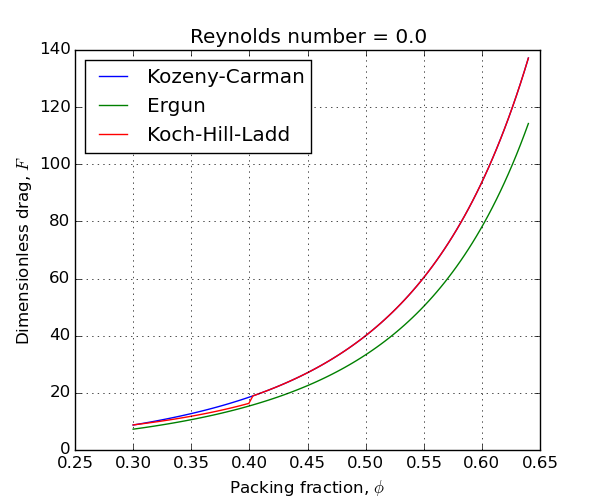
\includegraphics[width=\textwidth]{figures/pressure-drop-correlations/Re0.png}
    \end{subfigure}
    \begin{subfigure}[b]{0.45\textwidth}
        \centering
        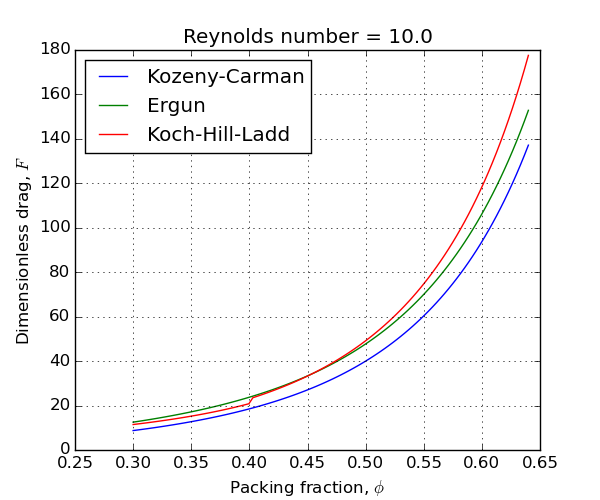
\includegraphics[width=\textwidth]{figures/pressure-drop-correlations/Re10.png}
    \end{subfigure}
    
    \begin{subfigure}[b]{0.45\textwidth}
        \centering
        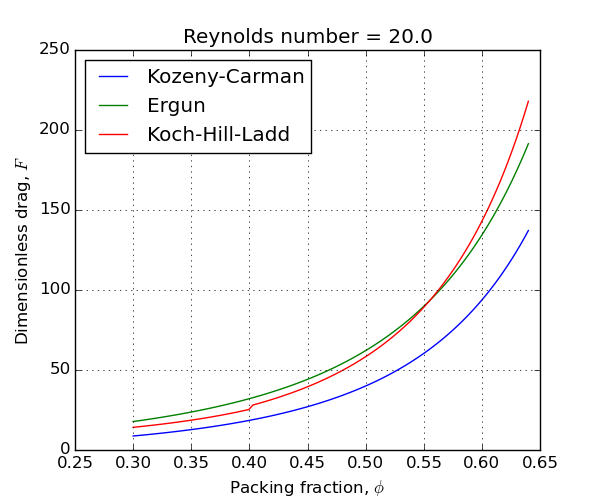
\includegraphics[width=\textwidth]{figures/pressure-drop-correlations/Re20.png}
    \end{subfigure}
    \begin{subfigure}[b]{0.45\textwidth}
        \centering
        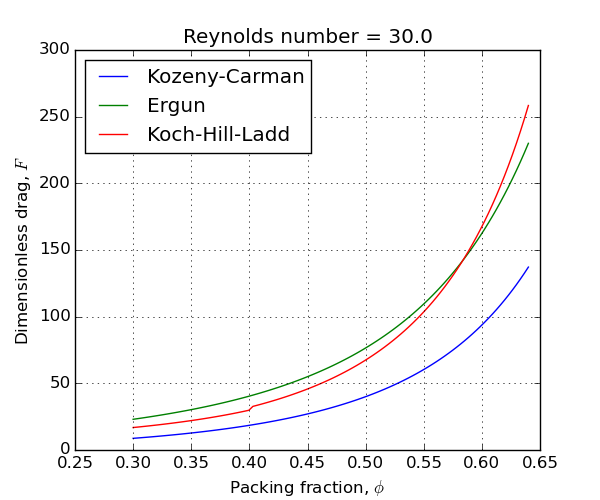
\includegraphics[width=\textwidth]{figures/pressure-drop-correlations/Re30.png}
    \end{subfigure}

    \begin{subfigure}[b]{0.45\textwidth}
        \centering
        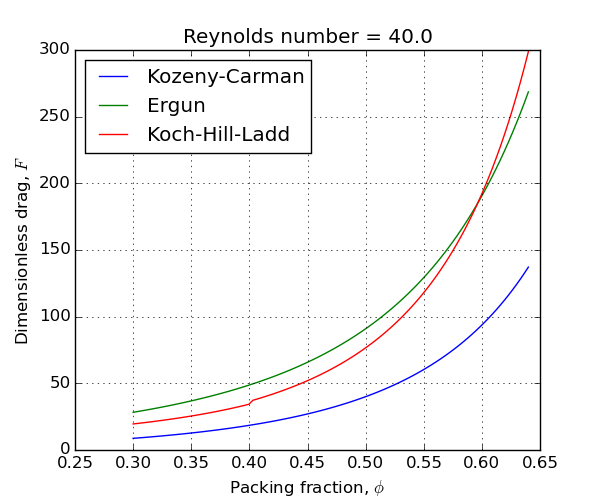
\includegraphics[width=\textwidth]{figures/pressure-drop-correlations/Re40.png}
    \end{subfigure}
    \begin{subfigure}[b]{0.45\textwidth}
        \centering
        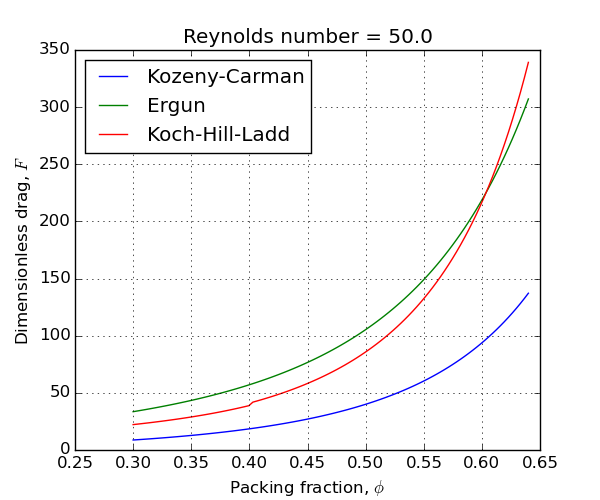
\includegraphics[width=\textwidth]{figures/pressure-drop-correlations/Re50.png}
    \end{subfigure}
    \caption{Comparison of pressure drop correlations over a range of packing fractions and Reynolds numbers.}
\label{fig:p-drop-correlations}
\end{figure}

\FloatBarrier




















%%%%%%%%%%%%%%%%%%%%%%%%%%%%%%%%%%%%%%%%%%%%%%%%%%%%%%%%%%%%%%%%%%%%%%%%%%%%%%%%%%%%%%%%%%%%%%%%%%%%%%%%%%%%
%%%%%%%%%%%%%%%%%%%%%%%%%%%%%%%%%%%%%%%%%%%%%%%%%%%%%%%%%%%%%%%%%%%%%%%%%%%%%%%%%%%%%%%%%%%%%%%%%%%%%%%%%%%%
%
% new section
%
%%%%%%%%%%%%%%%%%%%%%%%%%%%%%%%%%%%%%%%%%%%%%%%%%%%%%%%%%%%%%%%%%%%%%%%%%%%%%%%%%%%%%%%%%%%%%%%%%%%%%%%%%%%%
%%%%%%%%%%%%%%%%%%%%%%%%%%%%%%%%%%%%%%%%%%%%%%%%%%%%%%%%%%%%%%%%%%%%%%%%%%%%%%%%%%%%%%%%%%%%%%%%%%%%%%%%%%%%
\section{Status of Ceramic Breeder Modeling and Analysis}\label{sec:modeling-state}

Research efforts have been aimed at developing an understanding and characterization of thermomechanics of ceramic breeder pebble beds. Such an understanding is essential to providing confidence in performance and lifetime of ceramic breeder blanket designs. In particular, a significant effort of pebble bed thermomechanical studies is development of modeling simulation tools. In this section I will discuss the current state of modeling -- and experimental work feeding into modeling efforts -- for ceramic breeders of tritium.


%~~~~~~~~~~~~~~~~~~~~~~~~~~~~~~~~~~~~~~~~~~~~~~~~~~~~~~~~~~~~~~~~~~~~~~~~~~~~~~~~~~~~~~~~~~~~~~~~~~~~~~~~~~~
% new subsection
%~~~~~~~~~~~~~~~~~~~~~~~~~~~~~~~~~~~~~~~~~~~~~~~~~~~~~~~~~~~~~~~~~~~~~~~~~~~~~~~~~~~~~~~~~~~~~~~~~~~~~~~~~~~
\subsection{Experiments to Develop Constitutive Equations for Pebble Beds}


\begin{figure}
        \centering
        \begin{subfigure}[b]{\doubleimagewidth}
                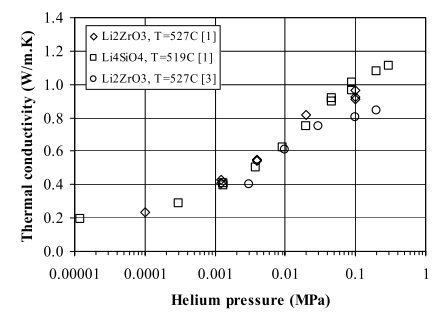
\includegraphics[width=\textwidth]{figures/keff-pressure}
                \caption{Effective conductivity of ceramic pebble beds is dependent on the pressure of the interstitial gas, a minimum of about $\keff = $\SI{0.2}{\watt\per\meter\per\kelvin} in vacuum.}
                \label{fig:keff-pressure}
        \end{subfigure}%
        
          %add desired spacing between images, e. g. ~, \quad, \qquad, \hfill etc.
          %(or a blank line to force the subfigure onto a new line)
        \begin{subfigure}[b]{\doubleimagewidth  }
                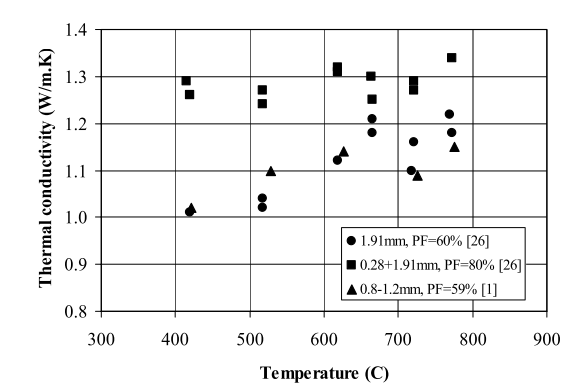
\includegraphics[width=\textwidth]{figures/lit-keff-exp}
                \caption{The effective conductivity of pebble beds is weakly dependent on external mechanical pressure and is always approximately $\keff = $\SI{1}{\watt\per\meter\kelvin} in helium.}
                \label{fig:keff-lit}
        \end{subfigure}
        \caption{Effective conductivity of lithium ceramics. Results from Ref.~\cite{Abou-Sena2005}}\label{fig:keff}
\end{figure}

Many experiments have been run to measure the effective thermal conductivity of a volume of ceramic pebbles. In \Cref{fig:keff}, the effective conductivity is seen to be strongly affected by the interstitial gas but weakly affected by the mechanical loads on the bed. The main conclusions to bear in mind from \Cref{fig:keff} are that: 1) the interstitial gas is an important transporter of heat in the bed and 2) the effective thermal conductivity of the pebble bed is low and will limit the size of the ceramic pebble bed volume to satisfy the temperature window mentioned above.



% Reimann and FZK experiments ~~~~~~~~~~~~~~~~~~
Reimann\etal~have conducted an extensive experimental study of stress-strain relations of ceramic breeder pebble beds using an oedometric test apparatus \cite{Piazza2002811,Reimann:2002kl,Reimann:2003qc,Reimann:2002mi,Reimann:2001il}. The most significant macroscopic experimental phenomena witnessed in pebble beds is an irreversible plastic strain when load is removed, a non-linear elasticity, a pressure-dependent plasticity, and volumetric creep.  A particularly noticeable feature, clearly demonstrated in Fig.~\ref{fig:mti}, is the reduced amount of irreversible strain when subjected to additional loading cycles after the first unloading. This may suggest the existence of a semi-equilibrium packing state in the pebble bed which can be reached after applying a pre-load to account for the large strain in the first cycle of a pebble bed. This semi-equilibrium packing state is a feature which may be advantageous for use in a fusion reactor.

To study temperature effects in Reimann's studies, beds are freely heated to desired working temperatures before pressure load is applied. Under the same loading condition, beds behave much softer at higher temperatures. The bed stiffens as the pressure increases. An illustration of this phenomenon is presented in Fig.~\ref{fig:UCT} for a lithium orthosilicate pebble bed between \SIrange{50}{850}{\celsius}. At higher temperatures (such as > \SI{650}{\celsius}), a creep-like behavior becomes apparent. Creep behavior allows the pebble bed to relax and sustain higher stresses, however at eleveated temperatures we must keep in mind issues of surface sintering of pebbles. The data was used to correlate creep rate as a function of temperature, stress, and time for both lithium orthosilicate, lithium metatitanate, and beryllium pebble beds \cite{Buhler:2002qf,Reimann:2001il,Reimann2005}.


\begin{figure}[t!]
    \centering
    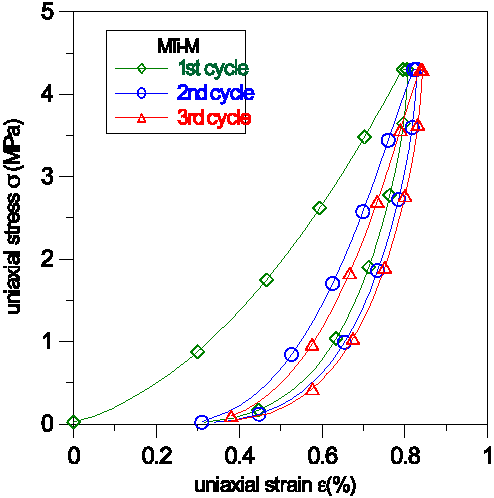
\includegraphics[width=\singleimagewidth]{figures/Fig-1}
    \caption{Example of uniaxial compression testing results for lithium metatitanate pebble bed \cite{vanderlaan2011}.}
    \label{fig:mti}
\end{figure}

\begin{figure}[t!]
    \centering
    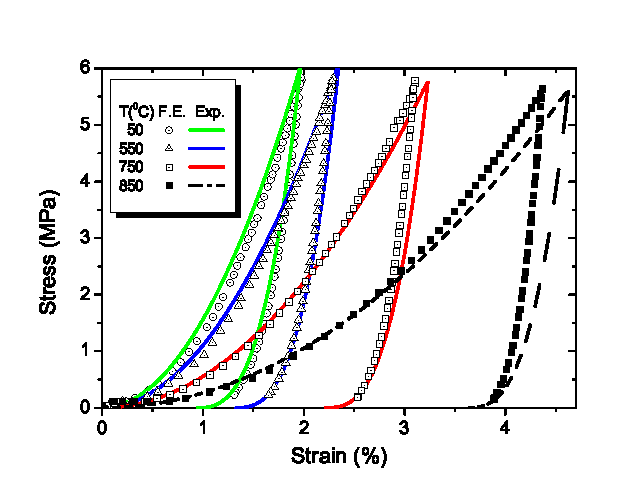
\includegraphics[width=\singleimagewidth]{figures/Fig-2}
    \caption{Example of uniaxial compression testing results compared with predictions from material constitutive equations for lithium orthosilicate pebble beds at different temperatures \cite{Gan:2008kx}.}
    \label{fig:UCT}
\end{figure}



% Japanese experiments~~~~~~~~~~~~~~~~~~~~~~~~~~~~~
Coming from the standpoint that strain in a pebble bed is induced by thermal expansion, an experiment was conducted to characterize the pebble bed thermal expansion coefficient \cite{Tanigawa:2007fc}.  The thermal expansion coefficient of a packed \lit~pebble bed is measured under a compressive load of 0.1MPa.  The study concludes that for beds with packing factors of 65.3 to 68.5\%, the average thermal expansion coefficient was $(1.4\pm0.2)\times10^{-5}K^{-1}$. This thermal expansion coefficient of the pebble bed was equal to 78\% of that for the bulk material under the conditions used in the study. The reduction in thermal expansion coefficient is less significant than that of the effective modulus, which is more than 2 orders of magnitude smaller than the bulk value. 


The effect of thermal cycling on the packing state is of interest; in particular, it is foreseen that the ITER TBM will be subjected to such conditions. The question that arises is whether a void region will be created under thermal-cyclic loading due to the differential rates of expansion and contraction of the pebble bed and structural containing wall. This uncertainty was first addressed in an experimental set-up involving Li$_2$TiO$_3$ pebbles enclosed by two Kovar flanges while sandwiched between two commercial-grade CVD silicon carbide discs \cite{Calderoni:2006ye}. The set-up allows for generating a high stress through large differential in thermal expansion coefficients. The experimental results indicate that high thermal stresses and deformations are present during the initial thermal cycle of the assembled test article, but are successively alleviated due to a combination of pebble re-arrangement within the bed and creep induced deformation. This suggests that a few thermal cycles under a controlled atmosphere and a compressive load before final assembly of blanket sections would mitigate the severity of the thermal stresses during start-up. This is also shown in a later experiment, in which the increment of compression decreased with each heating cycle and became negligible after 30 cycles \cite{Tanigawa:2010cr}. Extrapolating the finding to a prototypical blanket breeder pebble bed design, the study concludes that for a height of 1 m long pebble bed, a 51 mm high cavity may be generated at the top of the bed with an initial packing of 65\% under thermal cyclic operations.  


% UCLA experiments ~~~~~~~~~~~~~~~~~~~~~~~~~~~~~~~~~~~~~~~
Zhang\etal~ran similar cyclic pressure experiments to illuminate the existence of more steady stress-strain responses of packed beds under different pressures. 



\subsubsection{Post-irradiation experiments at Petten}
The pebble bed assemblies (PBA) experiment is designed to study the effect of neutron irradiation on the thermomechanical behavior of a ceramic breeder pebble-bed under DEMO representative thermomechanical loads \cite{Magielsen2007}. This was accomplished via analysis of changes of the in-pile temperature profiles during irradiation as wall as from the post irradiation examination of the pebble bed in the Hot Cells. Within the assemblies, there are four test elements; each resembling a small-scale mock-up of a HCPB TBM with a ceramic breeder pebble bed sandwiched between two beryllium pebble beds. Before irradiation, the beds are pre-compacted with a compressive load of 3 MPa to ensure good settling and contact.  

FEM analysis was performed to study pre-compaction procedures.  During progressive irradiation, temperatures are recorded at several locations in the ceramic breeder bed as well as other critical positions. Reviewing the recorded temperature data, when comparing the temperature in the center of the ceramic breeder pebble bed during later cycles and earlier cycles there appears to be a decrease in temperature for the exact same environmental conditions. Changes in the pebble beds and their characteristics are examined both in-pile by neutron radiography and out-of-pile by e.g. SEM during post-irradiation examination (PIE). The estimated bed height reduction from neutron radiographies over the course of the irradiation has shown 3\% of creep compaction. 

A pebble bed experiencing creep compaction is both becoming more dense as well seeing more-developed inter-pebble conduction paths. The effective thermal conductivity for a creep-compacted ceramic pebble bed is thus expected to be higher than a standard ceramic pebble bed. This phenomenon results in lower temperature gradients and a lower overall temperature magnitude, which is precisely what was observed in the experiment over the course of the cycling. 

During PIE, various microscopy preparation techniques are used to study the deformation state of the pebble beds (signs of creep compaction and sintering), formation of gas gaps between the pebble beds and structural materials, and the interaction layers between eurofer-ceramic and eurofer-beryllium. 

Figure~\ref{fig:pba} shows the cross-section of \lit~pebbles (left) and \lis~pebbles (right) post irradiation. Evident in the images is sintering of the lithium titanite and significant fracturing of the lithium orthosilicate pebbles. Importantly, however, it must be noted that the pebble beds performed reliably in spite of the changes displayed in these images cite{magielsen2011}. 


\begin{figure}[t!]
\centering
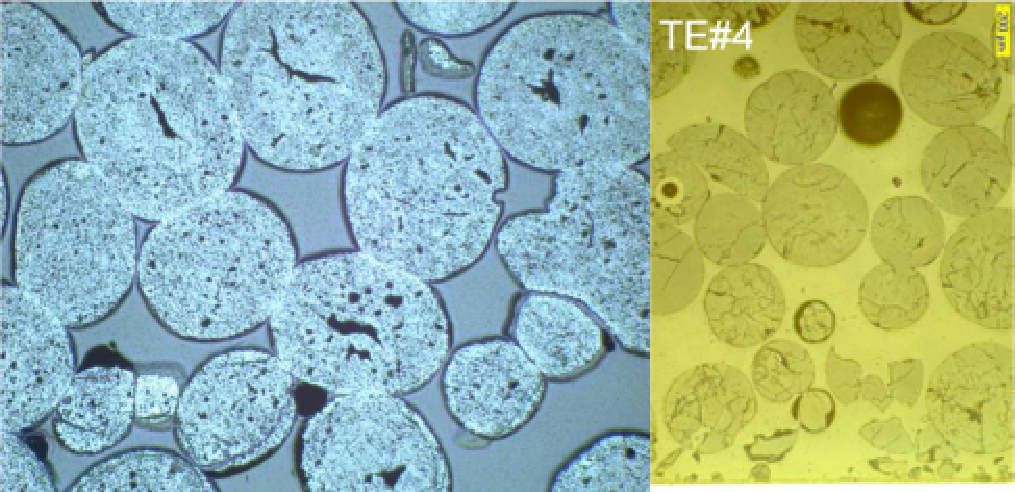
\includegraphics[width=\singleimagewidth]{figures/Fig-10}
\caption{Notable features of irradiated Li$_2$TiO$_3$ and Li$_4$SiO$_4$ pebble beds from PBAcite{magielsen2011}. (Left) Demonstration of significant sintering of Li$_2$TiO$_3$ pebbles with no fracturing; the visible cracks originated from production and handling. (Right) Demonstration of cracking of Li$_4$SiO$_4$ pebbles.}
\label{fig:pba}
\end{figure}



%~~~~~~~~~~~~~~~~~~~~~~~~~~~~~~~~~~~~~~~~~~~~~~~~~~~~~~~~~~~~~~~~~~~~~~~~~~~~~~~~~~~~~~~~~~~~~~~~~~~~~~~~~~~
% new subsection
%~~~~~~~~~~~~~~~~~~~~~~~~~~~~~~~~~~~~~~~~~~~~~~~~~~~~~~~~~~~~~~~~~~~~~~~~~~~~~~~~~~~~~~~~~~~~~~~~~~~~~~~~~~~
\subsection{Continuum Modeling of Granular Material for Solid Breeders}
When we consider beds of granular material from the standpoint of engineering continuum mechanics, packed beds cannot be adequately described by traditional models of either solids or liquids alone. Under compression, a packed bed responds like a solid with non-linear elasticity and a plasticity that is history-dependent. At the same time, the packed bed can obviously not support any tensile pressure and will often behave as an extremely viscous liquid as it may fill in voids under just the force of gravity. Nevertheless, phenomenological models, derived from the volumes of collected data, have been developed, using effective material properties for the ceramic pebble bed, that describe the pebble beds in an Eulerian manner that provide reliable information on the initial states of breeder volumes in the fusion reactor environment and allow reasonable design predictions of the Thermomechanics of the breeding blanket. 

In spite of the shortcomings of a continuum approach, it is the only option which currently allows treatment of the pebble beds with standard finite element modeling (FEM) that can be scaled up to the breeder system. To employ FEM, mathematical models written in terms of average quantities and containing effective parameters are used. These models deduce a set of constitutive equations to be implemented in the framework of a finite element code.  There are two major variants of phenomenological modeling approaches developed among institutions, including: (1) A non-linear elastic model and a modified Drucker-Prager-Cap theory for plastic strain \cite{Gan2007189,fokkens2003}; and (2) A hyper-porous non-linear elastic model and a Gurson model for the plastic model \cite{DellOrco:2007hc,DellOrco:2010zr,DiMaio20081287}. Another approach was taken by Ref.\cite{fokkens2003} wherein the authors employed two different elasticity laws for the loading and unloading branches. Alongside the development of the modeling techniques, several large scale pebble bed Thermomechanics experiments were conducted. These experiments were intended to reveal the underlined thermomechanical characteristics of ceramic breeder pebble beds, and provide data for benchmarking the developed models. The vast amount of work done on modeling the pebble beds in the FEM framework can be found in literature. \cite{DellOrco:2007hc,DellOrco:2010zr,DiMaio20101234,Gan2007189,Gan2007189,Gan:2009vn,Gan:2010lh,Gan:2010kc,DellOrco:2007hc,DellOrco:2010zr,DiMaio20101234,Gan2007189,DellOrco:2007hc,DiMaio20101234} A study was also published in 2012 that summarized, compared, and highlighted features of the models under development at the time.\cite{ying2011isfnt}



%~~~~~~~~~~~~~~~~~~~~~~~~~~~~~~~~~~~~~~~~~~~~~~~~~~~~~~~~~~~~~~~~~~~~~~~~~~~~~~~~~~~~~~~~~~~~~~~~~~~~~~~~~~~
% new subsection
%~~~~~~~~~~~~~~~~~~~~~~~~~~~~~~~~~~~~~~~~~~~~~~~~~~~~~~~~~~~~~~~~~~~~~~~~~~~~~~~~~~~~~~~~~~~~~~~~~~~~~~~~~~~
\subsection{Pebble Bed Modeling Benchmarks}

The constitutive equations developed for finite element models were derived from the uniaxial compression experiments, which are not fully representative of fusion operating conditions. A more prototypical experiment should subject a pebble bed to isostatic loading. This could be generated by either an in-pile pebble bed experiment or by making use of differential thermal expansion between a pebble bed and its containing structure. The latter has been attempted with several out-of-pile experiments launched by the HE-FUS 3 facility at ENEA Brasimone. The experiments investigated the thermomechanical behavior of pebble beds within geometry much more representative of current breeder designs. These include the medium-scale mock-up exercises of HELICA (HE-FUS3 Lithium Cassette) and HEXCALIBER (HE-FUS3 Experimental Cassette of Lithium Beryllium Pebble Beds) \cite{dellorco:2006,DiMaio20081287}. For those experiments, the pebble layers are heated by electric heaters, and temperature and displacement were measured.

\subsubsection{FZK Benchmarking}
FZK has performed validation of their FEM code against the data collected from the HELICA experiment \cite{Gan:2008kx}. They have also reported the results of simulations of HEXCALIBER but have, as yet, not directly validated against the collected experimental data \cite{Gan:2009vn}.

In the HELICA experiment, the pebble beds experienced six thermal ramps, each applied for an hour, and then the pebble beds were actively cooled with a helium flow. After cooling, the pebble beds were subjected to the another thermal ramp and the process was repeated. DIN reports\cite{dellorco:2006} that the pebble bed temperatures exhibited cyclical behavior. FZK simulated two cycles of the HELICA test and an example of the calculated results and experimental data are shown in Fig.~\ref{fig:FZK_HELICAa} and Fig.~\ref{fig:FZK_HELICAb}. In Fig.~\ref{fig:FZK_HELICAa} we see temperature histories at a particular location (100 mm from the first wall) during a loading-unloading cycle. The simulation results follow the temperature increase during the thermal ramps up until the seventh hour, then again follow the experimental data as the test rig is cooled with the helium coolant. Even with the two-dimensional simplification of the model, there is excellent agreement between calculations and measurements. In Fig.~\ref{fig:FZK_HELICAb} the displacement calculated by FZK is also in strong agreement with the average of measured displacements for the entire duration of the heating-cooling cycle. Because of the overwhelming amount of computer time necessary for the FZK model to complete a fully three-dimensional and transient simulation, the FZK computations of HELICA and HEXCALIBER are carried out in two dimensions; the helium temperature is chosen at an average value of measured inlet and outlet temperatures.

From FZK's numeric simulation arise several important observations: (i) a three-dimensional analysis would provide more detail, spatial temperature variation of e.g. coolants would likely explain much of the deviation between temperature profiles predicted by the simulation and measured in the HELICA experiment; (ii) gap formations, with sizes on the order of a pebble diameter, were detected at the interface of the first wall in ceramic beds; (iii) the maximum hydrostatic pressures seen in the ceramic bed are anticipated to be above the fracturing limit of the lithium ceramic. The consequences of some of these observations, if true and real, are severe enough that they merit careful attention. Gap formation and pebble failure (crush or fracturing) are important topics that must be considered in validation with future experiments.

\subsubsection{DIN Benchmarking}
Because of the characteristics of the DIN model, full three-dimensional simulations were capable of being relatively easily performed. In the framework of benchmarking efforts, DIN has performed validation of their model against experimental results of HELICA, shown in Fig.~\ref{fig:DIN_HELICA} as well as HEXCALIBER, shown in Fig.~\ref{fig:DIN_HEX}.

The results of the DIN model show also strong agreement to the experimental results of HELICA as demonstrated in one example of temperature histories shown in Fig.~\ref{fig:DIN_HELICA}. In this profile, the same location as that modeled by FZK (100 mm from the first wall) is simulated by DIN. The FEM simulations from DIN (Fig.~\ref{fig:DIN_HELICA}) are reported over the six-hour heating portion of a single heating ramp cycle of HELICA. When comparing the results from DIN with those of FZK (in Fig.~\ref{fig:FZK_HELICAa} and Fig.~\ref{fig:FZK_HELICAb}) we see the DIN model has slightly better predictive capabilities for the temperature histories. This may be due attributed to the three-dimensional variations in coolant temperature being captured by the DIN model. 


\begin{figure}[t!]
\centering
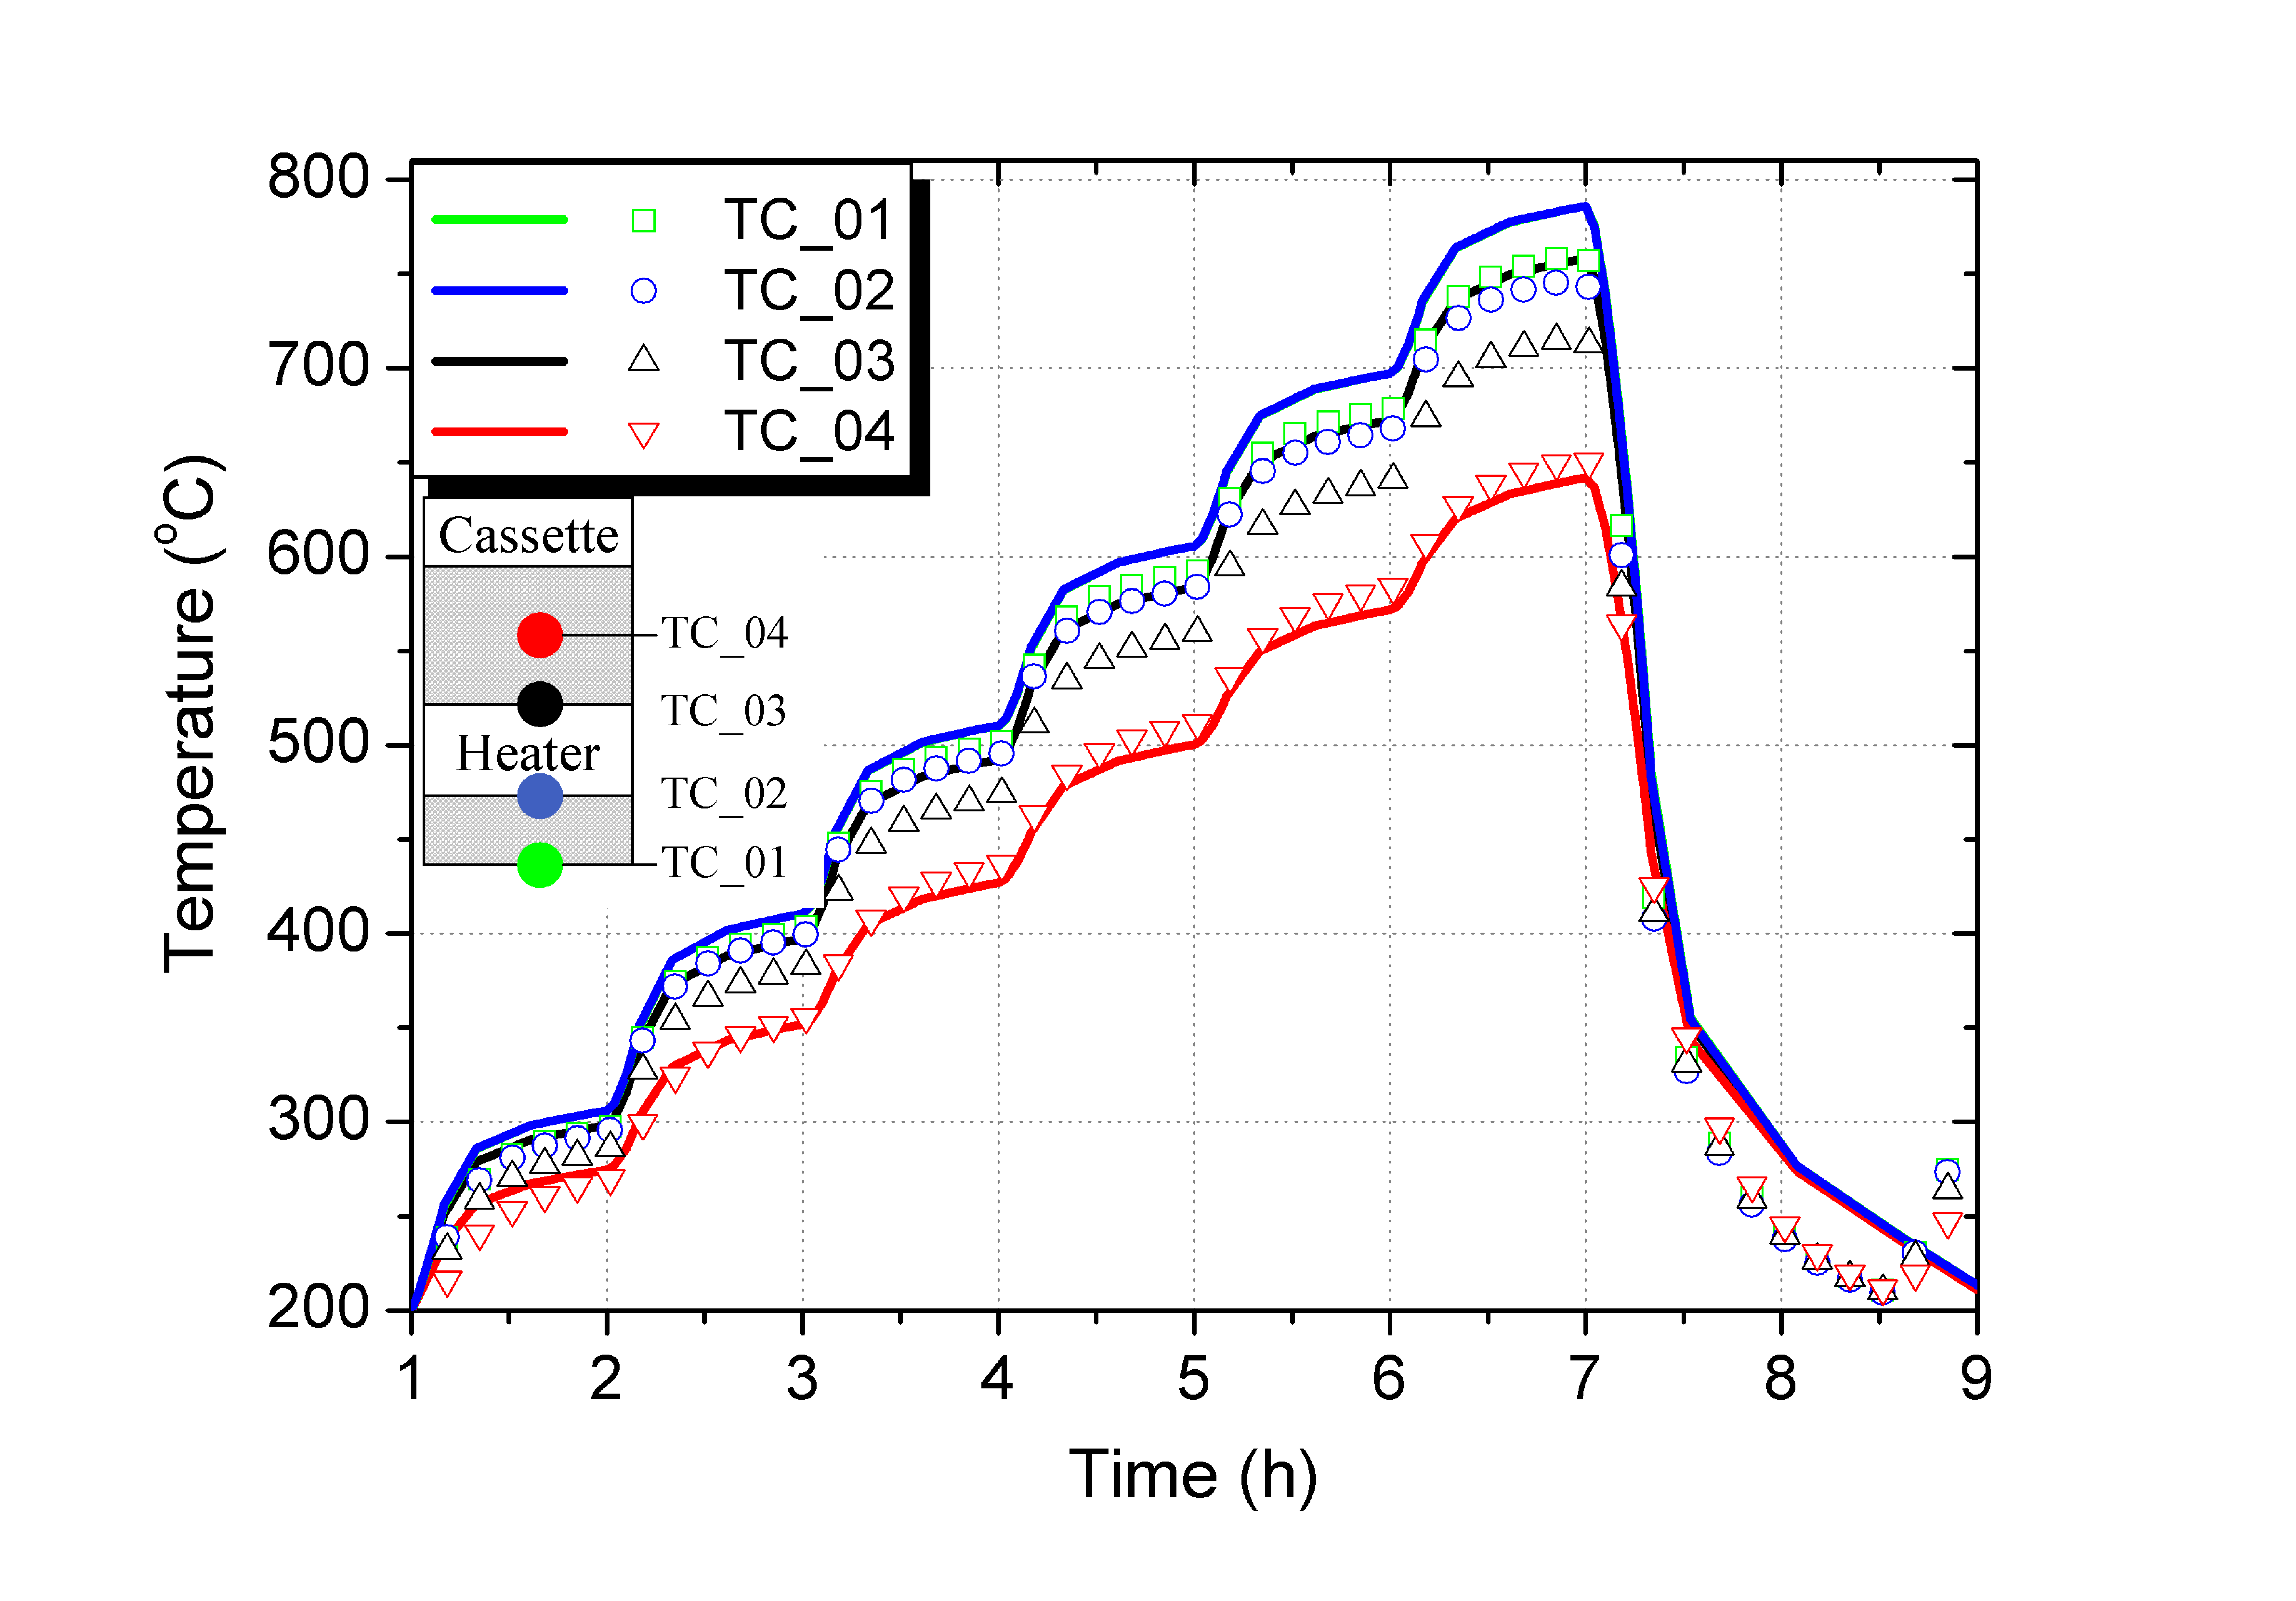
\includegraphics[width=\singleimagewidth]{figures/Fig-6}
\caption{Results of the FZK benchmarking with HELICA\cite{Gan:2009vn} showing temperature variations with time during a loading cycle (T in $^\circ$C) at 100 mm from FW.}\label{fig:FZK_HELICAa}
\end{figure}

\begin{figure}[t!]
\centering
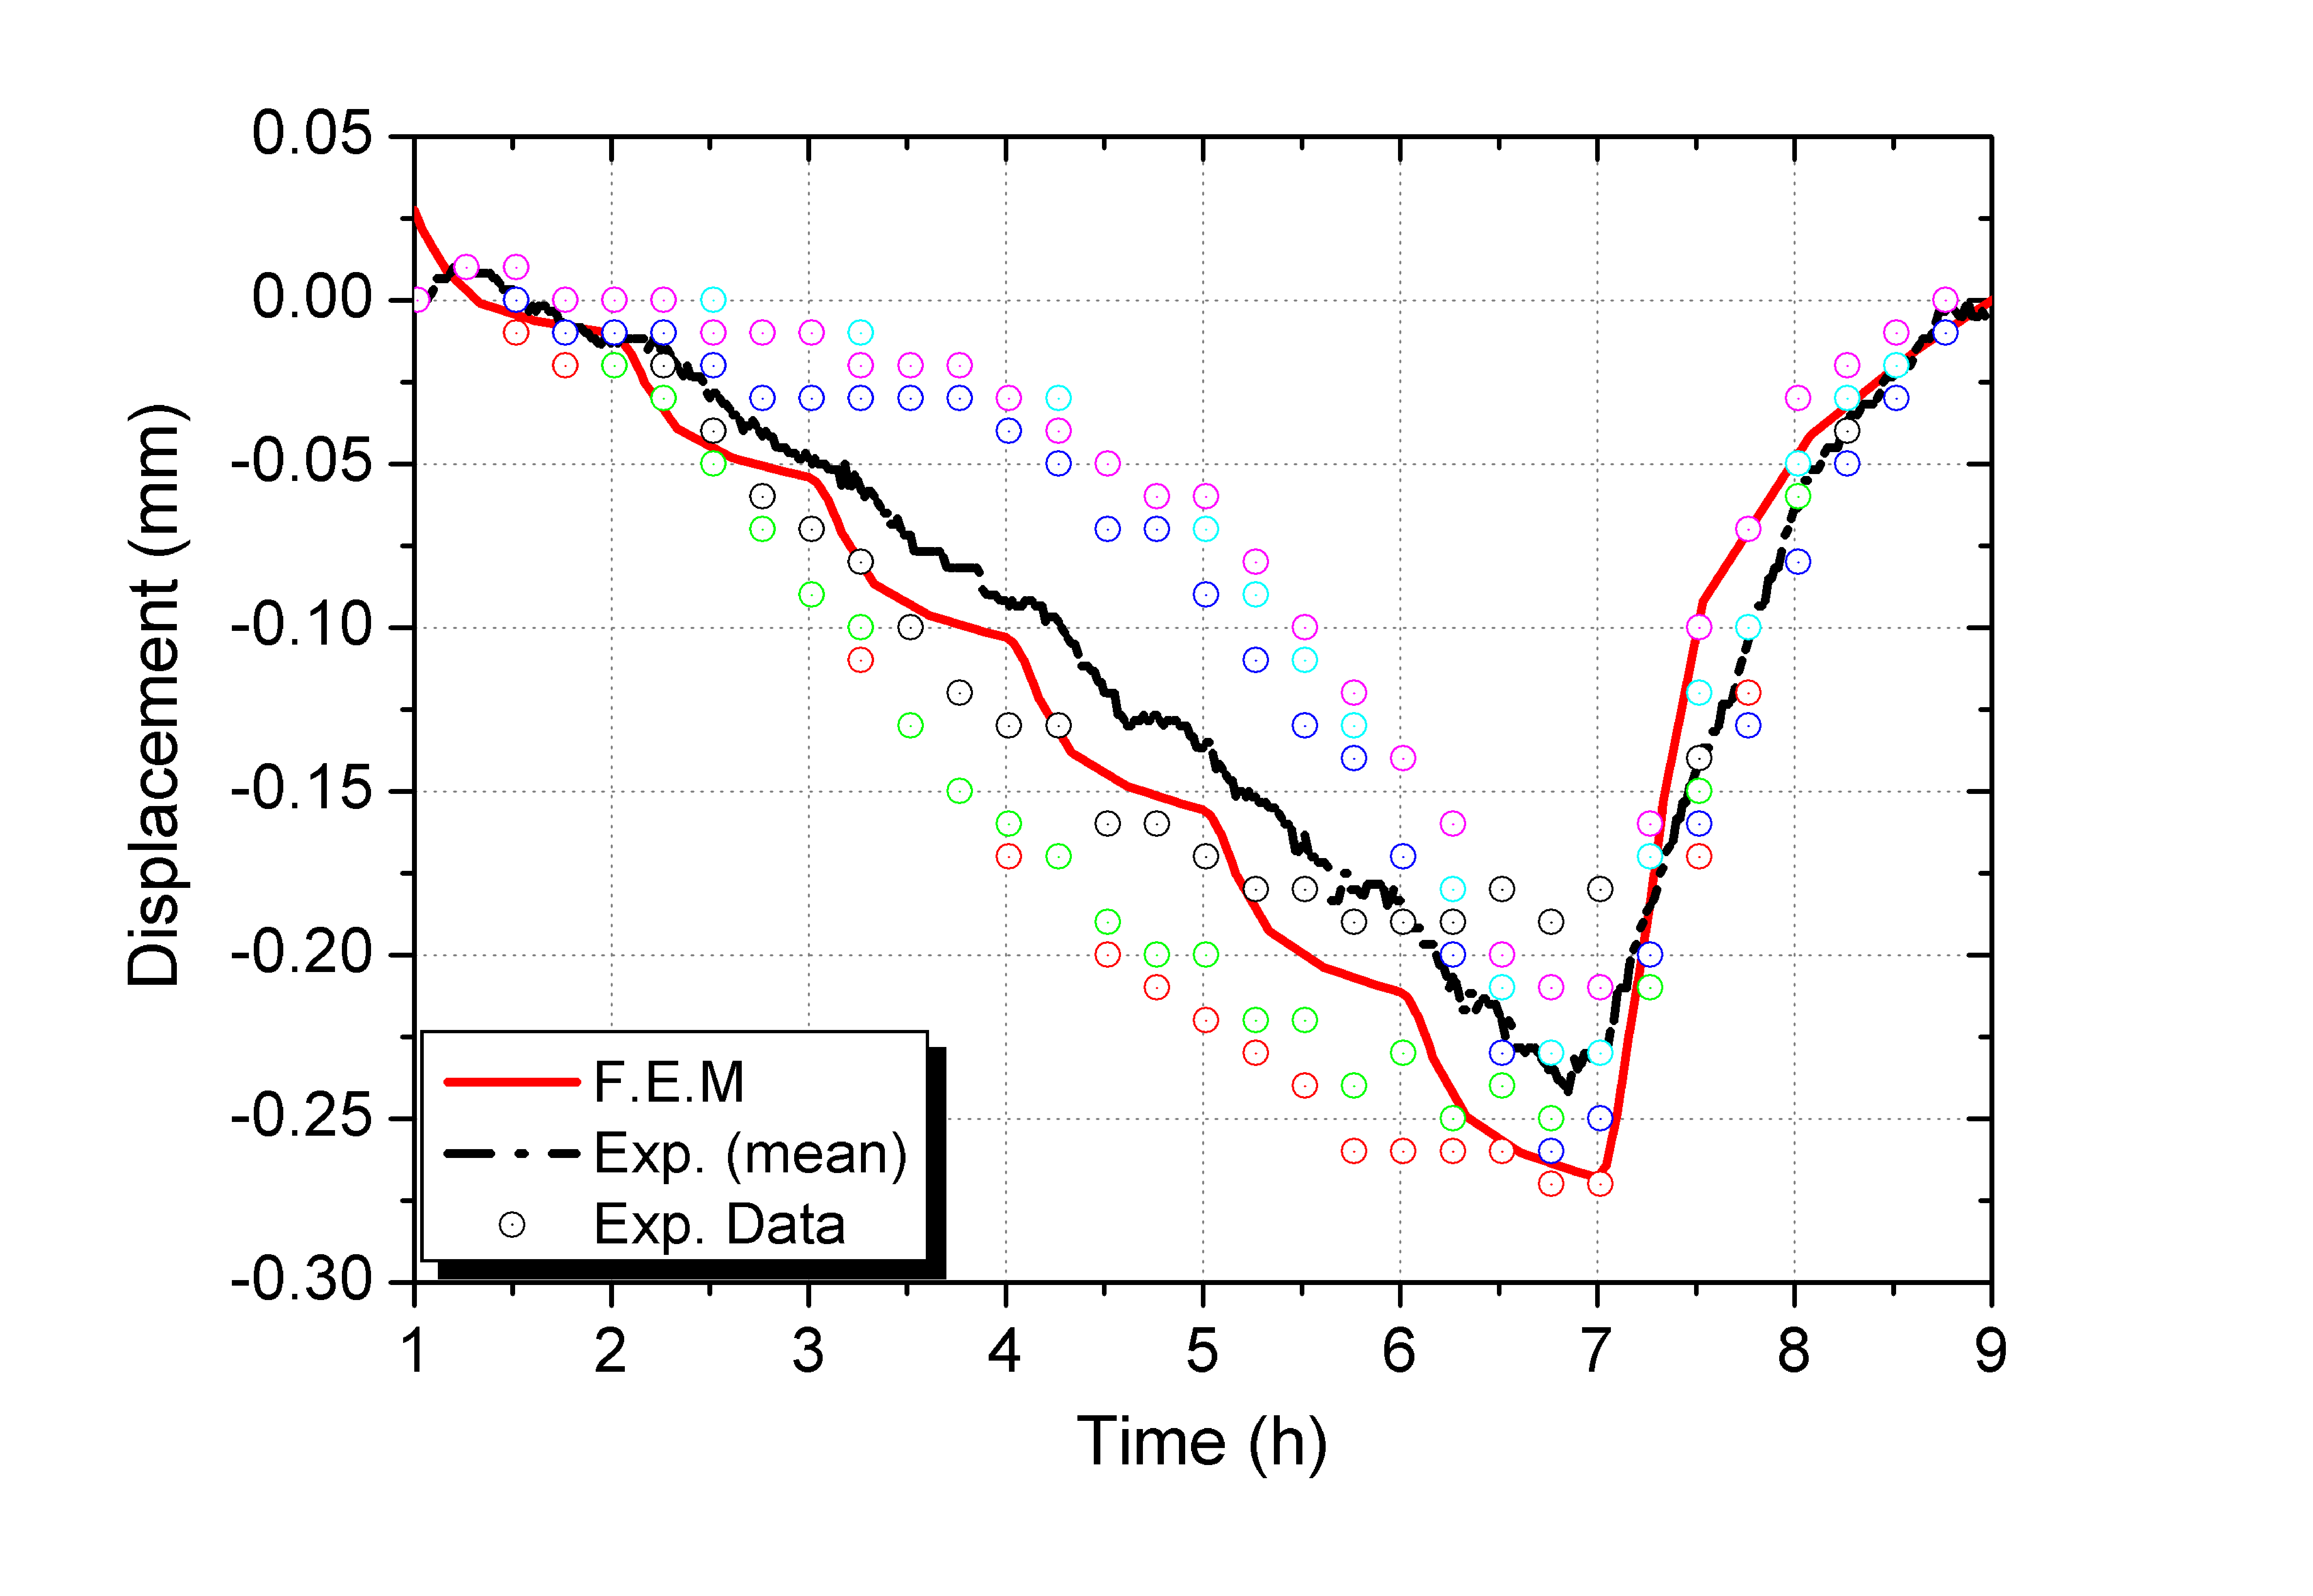
\includegraphics[width=\singleimagewidth]{figures/Fig-7}
\caption{Results of the FZK benchmarking with HELICA\cite{Gan:2009vn} showing a comparison of displacements (in mm) in HELICA between calculated and measured LVDT values.}
\label{fig:FZK_HELICAb}
\end{figure}

Unfortunately, the ambitions of HEXCALIBER were limited due to the crippling of several heaters. Nevertheless, the limited data was still used in efforts to validate the constitutive relationships of the DIN model. The temperature variations with time were the only major result reported by the ENEA Brasimone team, such as that shown in Fig.~\ref{fig:DIN_HEX}; mechanical results are still forthcoming from the research group. From the comparisons to experimental measurements in HELICA and HEXCALIBER it is encouraging to notice that even in the absence of a creep model, satisfactorily close agreement were seen between computation and measurement. So far, no detailed displacement comparisons have been made to experimental data.

Several important observations are also made from the results of the DIN simulation: (i) three-dimensional effects were important to calculations of the convective energy transport of the helium coolant; future models should continue to be analyzed in three-dimensions; (ii) DIN reports that in HELICA all ceramic beds experience a compressive force everywhere and no gap formation is ever detected. 

In summary, the benchmarking efforts have only recently begun in Europe. A typical pebble bed Thermomechanics simulation involves first calculating overall temperature fields of the blanket unit as it undergoes volumetric nuclear heating as well as cooling at the boundaries. The non-linear mechanical analysis is then performed for stress and strain estimations. However, since the effective thermal conductivity of the ceramic breeder pebble bed is, to some degree, dependent on strain, a coupled thermal and mechanical analysis is needed. Additional details on modeling steps can be found in Refs.~\cite{DellOrco:2010zr,DiMaio20081287,DiMaio20101234,Gan:2009vn,Gan:2010lh,dellorco:2006}. The two most developed models, from FZK and DIN, have had their results compared to experimental data and have thus far shown great promise. 

However, it must be noted that the benchmarking efforts are incomplete and inconsistencies between the two models must be explained as they move forward. For example, the model of FZK concluded that a gap appeared between the pebble bed and structural wall, however the model from DIN reported no gap formation. The existence of a gap between pebble bed and structural wall will negatively affect the ability to cool the pebble bed and thereby impact structural and tritium release properties of the bed. That such a discrepancy exists between calculated results of the models on such a critical feature warrants either more benchmarking efforts or a careful deconstruction of the constitutive equations to discover the source of the inconsistency. Future experiments aimed at benchmarking ought to focus on creating apparatus capable of expressing, among other things, when gap formation or pebble failure occurs.


\begin{figure}[t!]
    \centering
    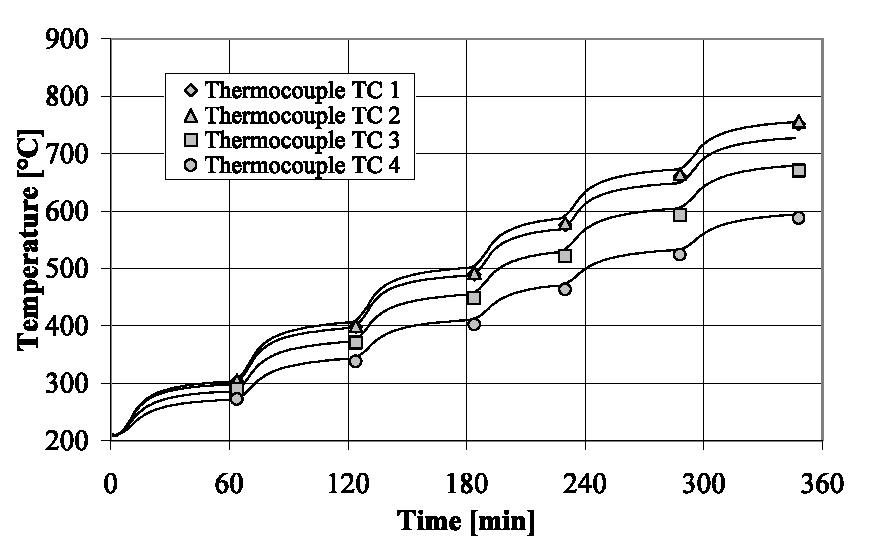
\includegraphics[width=\singleimagewidth]{figures/Fig-8}
    \caption{Exemplary results of the DIN benchmarking with HELICA: Temperature variations with time during a loading cycle at 100 mm from FW\cite{DellOrco:2007hc}.}
    \label{fig:DIN_HELICA}
\end{figure}


\begin{figure}[t!]
    \centering
    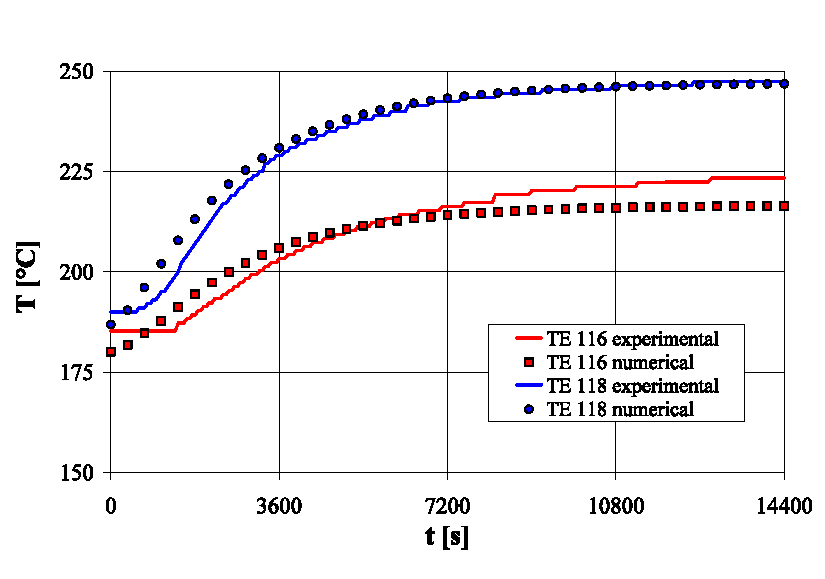
\includegraphics[width=\singleimagewidth]{figures/Fig-9}
    \caption{Exemplary results of the DIN benchmarking with HEXCALIBER : Temperature variations with time during a loading cycle within the first lithium-orthosilicate cell\cite{DellOrco:2010zr}.}
    \label{fig:DIN_HEX}
\end{figure}





%~~~~~~~~~~~~~~~~~~~~~~~~~~~~~~~~~~~~~~~~~~~~~~~~~~~~~~~~~~~~~~~~~~~~~~~~~~~~~~~~~~~~~~~~~~~~~~~~~~~~~~~~~~~
% new subsection
%~~~~~~~~~~~~~~~~~~~~~~~~~~~~~~~~~~~~~~~~~~~~~~~~~~~~~~~~~~~~~~~~~~~~~~~~~~~~~~~~~~~~~~~~~~~~~~~~~~~~~~~~~~~
\subsection{Discrete Element Method for Solid Breeders of Tritium}
However, current continuum models will be shown to be insufficient for capturing the evolving thermomechanics of the packed bed as bed resettling, individual grain crushing, and the helium purge influence the packing structure and inter-particle force networks in the bed. Thus in this dissertation I will approach the pebble bed from the microscopic scale of individual grains via the discrete element method to enable predictive capabilities for temperature profiles in ceramic breeder pebble beds with a helium purge gas -- even those experiencing bed resettling and grain crushing. Along the way, new constitutive relationships for material properties are discovered, fragmentation models are created, and new heat transfer models are incorporated.



Correlations for effective properties of heat transfer and the constitutive equations derived from experiments are, however, still incapable of accurate modeling of granular thermomechanics as the granular material evolves in time (based on creep, granular crushing, sintering, \textit{etc.}), thus many researchers of ceramic pebble beds began modeling with the grain-scale discrete element method (DEM). The last part of this chapter revolves around discussion of historical efforts of applying DEM to solid breeders and important results obtained.

A thorough review of the physics behind DEM will be given in \cref{sec:dem-studies}. For now, we will simply discuss some major results of the implementation of DEM in past solid breeder research.

The Discrete Element Method (DEM) introduced by~\cite{Cundall1979} has been shown to be a promising tool to study the behavior of granular systems through the interaction between the individual particles. DEM was first applied to study the micro-mechanical aspects of cyclic thermal loads on the relaxation of stress in pebble beds for fusion reactors.\cite{Lu2000b,Ying2002}. An iterative relaxation strategy of DEM was used to study the internal contact forces in a pebble bed under an external load by An\etal\cite{An20072233} The same DEM tools, and the insight provided by which, were also used to initiate DEM-based investigations of creep between pebbles under thermal and mechanical loads.\cite{An20071393} While An\etal~studied the pebble assemblies in rectangular and cylindrical containers bounded by a elastic walls, computational requirements prevented more than a few thousand particles in the ensemble with rigid walls.\cite{An20072233} Following An's work, the DEM torch was passed across the pond to researchers at KIT where they began to improve upon the initial studies begun at UCLA.

\begin{figure}[!ht]
    \centering
    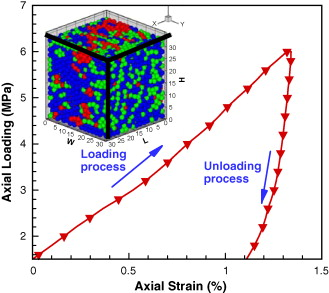
\includegraphics[width=\singleimagewidth]{figures/1-s2.0-S092037960700049X-gr1.jpg}
    \caption{Stress–strain behaviors of granular materials in a rectangular box under uniaxial compaction from DEM are qualitatively matched to behaviors seen experimentally.}
\label{fig:an-uniaxial-compression}
\end{figure}

The effect of packing factor, geometry of the assembly on the overall stress-strain response under uniaxial compression tests (UCT) has been thoroughly investigated.\cite{Gan:2010uq} Gan\etal~pebble assemblies in a cubic box with periodic boundary conditions to prevent the influence of boundaries dominating the ensemble response to loads.\cite{Gilabert2007} In the DEM uniaxial compression studies (see Fig.~\ref{fig:an-uniaxial-compression}), a non-linear stress-strain response and a characteristic residual strain after unloading (analogous to plastic strain in continuum systems) is observed akin to the experimental results.\cite{Reimann:2000tw} It was shown that the average coordination number, average normal contact force and the maximum normal contact force in the assembly has a unique functional relation (nonlinear, linear and linear, respectively) with the hydrostatic pressure or the applied pressure independent of the packing factor.\cite{Gan:2010uq,An20071393} These functional relations may be used as master curves for the micro-macro correspondence in the pebble bed Thermomechanics studies.

Recently, the effect of the pebble size distribution on the overall thermomechanical behavior of the pebble assembly is studied by Annabattula\etal\cite{Annabattula2011}. They consider the pebble size distribution of ceramic breeder pebbles (\lis) with a diameter range of $0.25\ \mathrm{mm}$-$0.65\ \mathrm{mm}$. Figure~\ref{fig:pebble-assembly-potential-energy} shows a binary pebble assembly in a periodic box. The colors indicate stored elastic strain energy of the pebble (red: maximum and blue: zero). The assembly has a maximum pebble radius $\rmax=0.25$ mm with the pebble size ratio $\rstar=\rmin/\rmax=0.6$, relative volume fraction $\vstar=\vmax/V=0.7$ and a packing factor $\eta=0.643$. The average stress in a granular assembly can be deduced from the contact forces between individual grains.


\begin{figure}[!ht]
    \centering
    \begin{minipage}{0.45\singleimagewidth}
    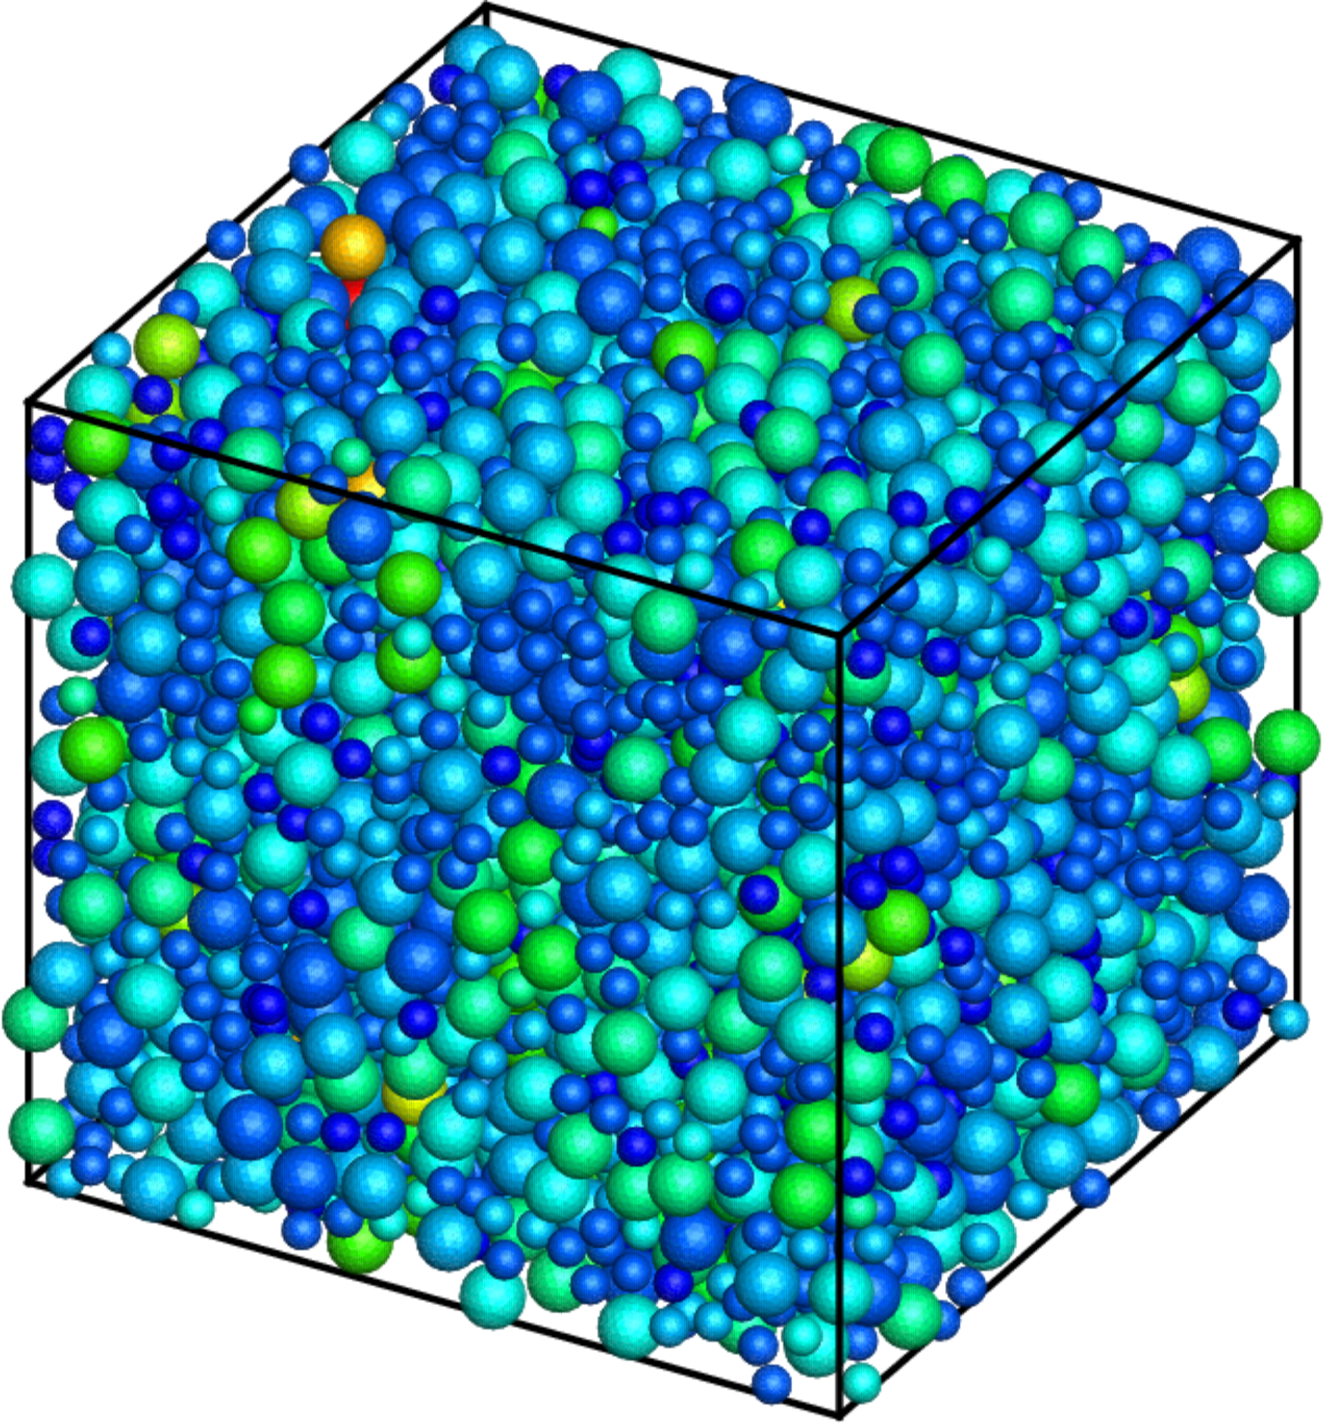
\includegraphics[width=6cm]{figures/Fig-3}
    \begin{picture}(15,15)(340,-120)
    \put(330,-80){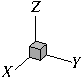
\includegraphics[scale=1]{figures/Fig-3b}}
    \end{picture}
    \end{minipage}
    \caption{A binary pebble assembly with $\rstar = 0.6$ and $\vstar=0.7$ showing the stored elastic energy of the pebbles at $\epsilon_{33}=1.5\%$; pebbles of radius $r_s$ (small) and $r_g$ (large).}
    \label{fig:pebble-assembly-potential-energy}
\end{figure}

Another aspect of interest in the study of mechanics of pebble beds is the crush behavior of individual pebbles and their impact on the over all pebble bed response. DEM was used to study the behavior of a crushable pebble assembly with the crush load data for \lis~pebbles (for individual pebbles) measured at KIT for pebbles of diameter 0.5 mm. 

A probabilistic method for analyzing the crush events of individual pebbles and a procedure with the combination of DEM and experimental data to obtain crush load probability has been reported by~\cite{Gan:2010kc}. Figure~\ref{fig:cdf_pebbles} shows the cumulative distribution function as a function of the hydrostatic pressure placed on the bed. The probability analysis, derived from DEM calculations, provides quantitative report of pebble crushing as a function of a specific hydrostatic pressure. The results of this analysis exemplify the growing strength of DEM techniques for analyses connecting global pebble bed loads to individual pebbles.

\begin{figure}[!ht]
  \centering
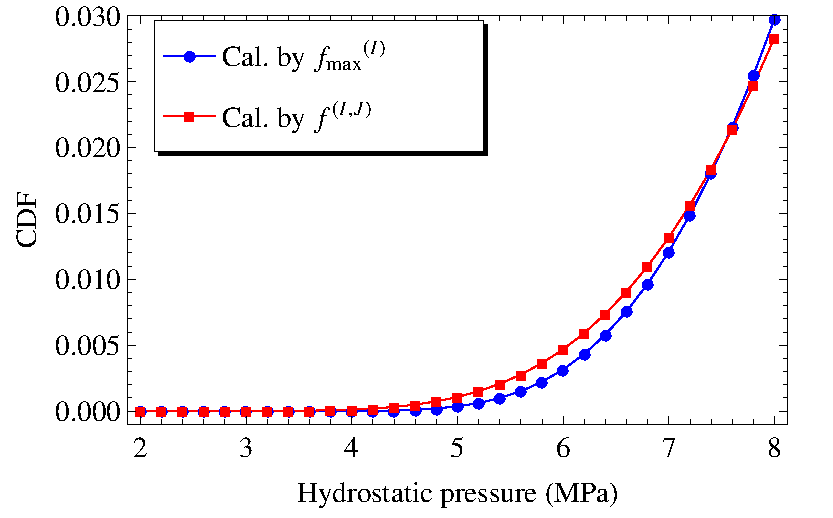
\includegraphics[width=\singleimagewidth]{figures/Fig-4}
 \caption{Cumulative distribution functions for crushing of individual pebbles inside the bed for as-fabricated pebbles, calculated by (1) maximum contact forces and (2) all inter-particle contact forces~\cite{Gan:2010kc}.}
 \label{fig:cdf_pebbles}
\end{figure}

However, it has been shown~\cite{Zhao2010,Zhao2011} that a criterion based on critical stored elastic energy is the most suitable criterion for describing the \lis~pebble failure. Hence, the crush load data (provided by fusion materials laboratory at KIT) has been transformed into equivalent elastic strain energy showing a Weibull distribution~\cite{Zhao2010}. This critical energy (randomly generated distribution) is used as the criterion for failure of pebbles in the DEM simulations. First, the assembly is loaded up to 3\% strain in uniaxial compression and then unloaded to a stress-free state. The elastic modulus of the pebble is reduced (from initial value to a small value of 1 kPa) with increase in elastic strain energy of the pebble according to a phenomenological damage accumulation law~cite{Annabattula2011b}. The damage state is frozen at the end of loading step and hence there will be no further damage accumulation in the unloading step. 

Figure.~\ref{fig:stress-strain-effect} shows the results for two types of damage law each with three different realizations. Each realization corresponds to a different random distribution of critical energies assigned to the pebbles in the assembly. The results do not show appreciable sensitivity to random distribution of energies. In the case of gradual damage law, the reduction of the elastic modulus of the pebble starts when the stored elastic energy reaches 50\% of the critical energy for that pebble and the elastic modulus reaches exponentially to its minimum value when the stored elastic energy reaches the critical energy prescribed. In the case of sudden damage this reduction starts at a much later stage when the stored elastic energy reaches 95\% of the critical energy of the pebble. Clearly, the assembly with a sudden damage accumulation shows a higher maximum strength compared to the gradual damage. In the case of the gradual damage, the pebbles start to degrade much earlier (at small strain) than in the case of sudden damage. Hence the critical number of pebbles to fail for the onset of maximum strength is reached earlier (at small strain) in gradual damage. It turns out that a mere 0.2\% pebbles is the critical number for the onset of maximum strength (stress plateau) observed.

\begin{figure}[!ht]
\centering
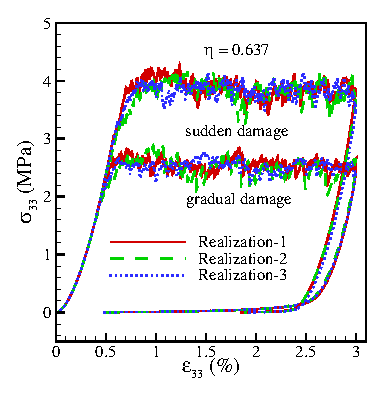
\includegraphics[width=\singleimagewidth]{figures/Fig-5}
\caption{Stress-Strain response of a granular assembly under uniaxial compression for two different damage evolution laws (gradual and sudden). Each damage evolution criterion is simulated with three different realizations of randomly prescribed critical failure energy for individual pebbles following Weibull distribution.}
\label{fig:stress-strain-effect}
\end{figure}

The nature of damage evolution influences the maximum strength and strain at which the maximum strength is attained while the critical number of failed pebbles for this saturation is independent of the damage evolution law (also see~\cite{Zhao2010}). Also note that the high frequency oscillations during loading in the stress-plateau region represent the failure of new pebbles. The current analysis also shows a creep-like behavior of the stress-strain response and hence the stress-plateaus observed in the experiments~\cite{Reimann:2000tw} may indicate the presence of pebble crushing in addition to the thermal creep mechanism. Furthermore, the residual strain after unloading is large for the system with sudden damage than the system with gradual damage. It should be noted that the assembly with gradual damage has more number of damaged pebbles at the end of loading (at 3\% strain) making the assembly more compliant than in the case of sudden damage. 








%~~~~~~~~~~~~~~~~~~~~~~~~~~~~~~~~~~~~~~~~~~~~~~~~~~~~~~~~~~~~~~~~~~~~~~~~~~~~~~~~~~~~~~~~~~~~~~~~~~~~~~~~~~~
% new subsection
%~~~~~~~~~~~~~~~~~~~~~~~~~~~~~~~~~~~~~~~~~~~~~~~~~~~~~~~~~~~~~~~~~~~~~~~~~~~~~~~~~~~~~~~~~~~~~~~~~~~~~~~~~~~
\subsection{Conclusions on Solid Breeder Granular Material Literature Review}
A good deal of progress has been made in the field of ceramic pebble bed analysis. Owing to the multi-scale nature of pebble beds, it is unavoidable that multi-scale models are necessary. In this framework, the continuum modeling approach using FEM and empirically derived material constitutive equations is capable of correctly characterizing the stress load to which a breeder pebble bed unit may be subject during reactor operation. The DEM approach analyzes this load and determines the possibility of pebble bed morphological changes; i.e. pebble damage based on the crush load data of pebbles, the degree of sintering depending on the local contact stress and temperature fields, and creep relaxation of contacts. It is only with the combined analysis of particle-scale information from DEM and system-scale information from FEM that warrants a high confidence of success to the assembly and design of breeder units in a blanket.  Experiments should also be conducted to assess the manner of pebble relocations and packing rearrangement when morphological evolution of the pebble bed occurs. It is important to learn if the breeder unit will continue to function in accord with the original design goals under all complex operating conditions.  The ultimate objectives of the pebble bed Thermomechanics are: to delineate a near-equilibrium packing state as the initial state, quantify breeder unit Thermomechanics parameters during operations, understand how these properties evolve as topographical changes happen in the packing, and ensure breeder functions as it is intended to in the fusion operational phase spaces.


Lastly, no predictive tool is possible without solid validation attempts. The benchmark experiments performed up to now were either too limited in scope or practice. New experiments must be performed that can provide reliable data with which to compare numerical results. Fortunately, a new experimental effort out of KIT has been initiated.\cite{Hernandez2014} The experiment shows great promise at reproducing volumetric heating profiles with substantial data collection efforts. The preliminary results are very promising.


